% ============================================================================
% preliminary_results.tex
% Master thesis preliminary results on the MTU15 (intraday and day-ahead)
% reforms: effect on bids, prices and quantities, using the critical/flat
% hour-class identification strategy. Companion: descriptive_facts.tex.
% ============================================================================

\documentclass[11pt]{article}

\usepackage[margin=2.4cm]{geometry}
\usepackage{graphicx}
\usepackage{amsmath, amssymb}
\usepackage{booktabs}
\usepackage{array}
\usepackage{longtable}
\usepackage{multirow}
\usepackage[table]{xcolor}
\usepackage{tikz}
\usetikzlibrary{arrows.meta, positioning, decorations.pathreplacing}
\usepackage[round,authoryear]{natbib}
\usepackage{hyperref}
\hypersetup{colorlinks=true, linkcolor=blue!50!black, citecolor=black, urlcolor=blue!50!black}
\usepackage{microtype}
\usepackage{enumitem}
\setlist[itemize]{leftmargin=*, itemsep=5pt, topsep=5pt}
\usepackage{titlesec}
\usepackage{float}
\usepackage[font=footnotesize, labelfont=bf, margin=1.2cm]{caption}
\titlespacing*{\section}{0pt}{18pt}{10pt}
\titlespacing*{\subsection}{0pt}{12pt}{6pt}
\titlespacing*{\subsubsection}{0pt}{10pt}{4pt}
\titleformat*{\subsubsection}{\bfseries\itshape}
\titlespacing*{\paragraph}{0pt}{10pt}{8pt}
\renewcommand{\arraystretch}{1.18}
\linespread{1.12}

\usepackage[most]{tcolorbox}
\newtcolorbox{takeaway}{
  enhanced,
  colback=black!3,
  colframe=black!55,
  boxrule=0.5pt,
  arc=2pt,
  left=8pt, right=8pt, top=5pt, bottom=5pt,
  before skip=6pt, after skip=8pt,
}

\graphicspath{{../../figures/thesis/}{../../figures/working/}}

\title{Preliminary results master thesis}
\author{\normalsize Pablo Paramio P\'erez}
\date{\normalsize\today}

\begin{document}
\maketitle
\vspace{-0.8cm}

{\hypersetup{linkcolor=black}\tableofcontents}
\vspace{6pt}
\hrule
\vspace{6pt}

\section*{1. Setup: outcomes, windows, and seasonal control}
\addcontentsline{toc}{section}{1. Setup: outcomes, windows, and seasonal control}
\phantomsection\label{sec:setup}

\paragraph{(Two) reforms.} The Spanish wholesale electricity market shifted from a 60-minute to a 15-minute market time unit in two steps: \textbf{ID15} (2025-03-19, intraday auctions and continuous market) and \textbf{DA15} (2025-10-01, day-ahead). After each reform there are four periods per clock-hour; before, one. A third granularity reform, \textbf{ISP15} (2024-12-11), moved REE's settlement period\footnote{There are penalizations for the units when they deviate from their scheduled production.} from 60 to 15 minutes but left the OMIE contract grid unchanged. The \emph{operaci\'on reforzada} regulatory stance (REE's post-blackout reinforced operation, continuous from 2025-04-28) is a continuous confound that forces CCGT post-dayahead inclusion; tight pre/post windows around each reform date hold its level constant within each arm. Figure~\ref{fig:bid_internal:timeline} summarises the full timeline, including other reforms that are not directly relevant for our research question but are important for context.

\begin{figure}[H]
\centering
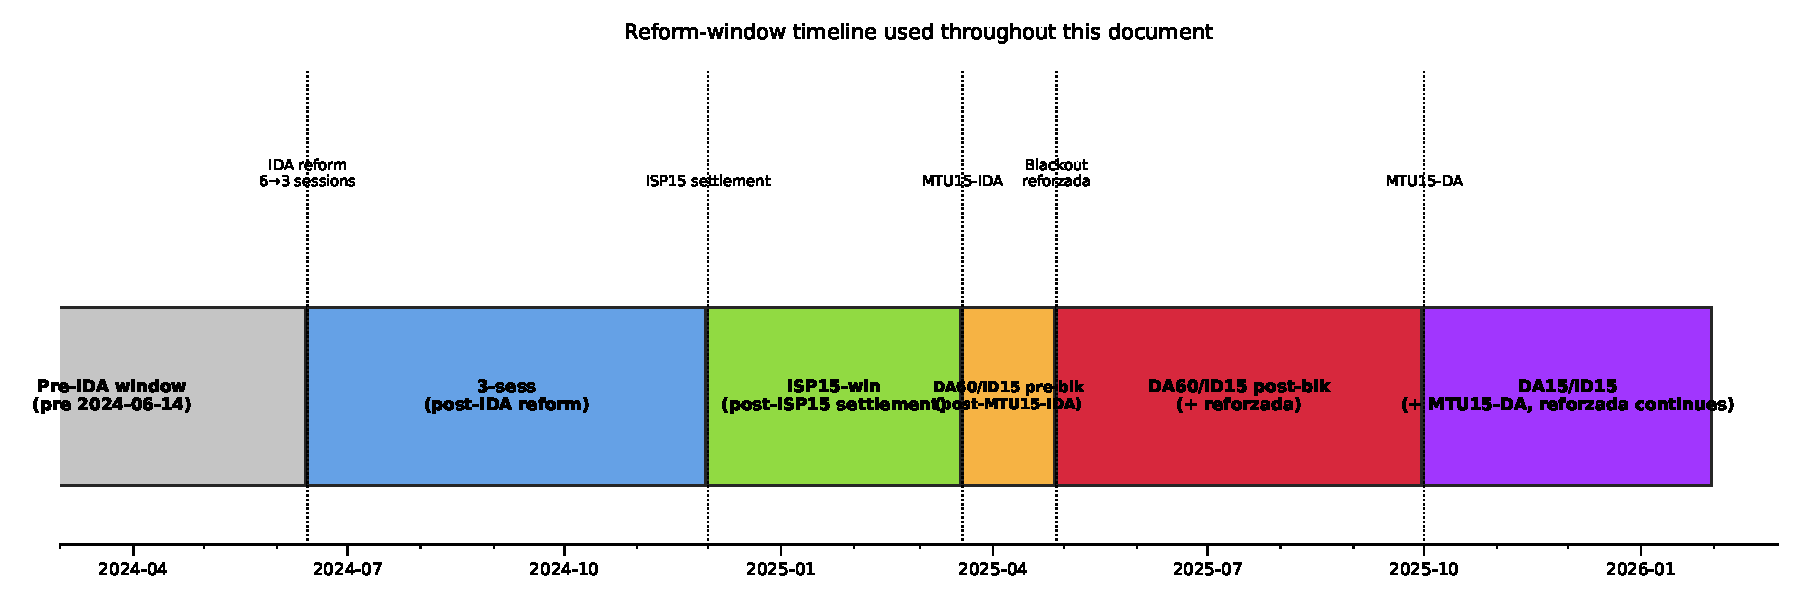
\includegraphics[width=0.98\textwidth]{../../figures/thesis/timeline_reform_windows.pdf}
\caption{\textbf{Full reform-window timeline.} Five named windows partition the post-2024-06-14 sample; the pre-IDA window is the baseline regime. Dotted vertical lines mark the five reform dates that produce the window boundaries.}
\label{fig:bid_internal:timeline}
\end{figure}

\paragraph{Variables.} Each (unit $u$, date $d$, period $p$) sell offer is a tranche ladder $\{(p_k, \Delta q_k)\}_{k=1}^{K_{u,d,p}}$ sorted by ascending price, where $p_k$ is the bid price (EUR/MWh) and $\Delta q_k$ is the \emph{incremental} MW added to the unit's step supply function at $p_k$\footnote{Following OMIE \emph{Potencia} field in \textit{ficheros OMIE v1.37} \S 5.1.4.2. $\Delta q_k$ is the marginal MW at tranche $k$; the unit's total offered capacity in the period is $\sum_k \Delta q_k$, and the cumulative supply at any price $p$ is $S(p)=\sum_{k:\,p_k\le p}\Delta q_k$.}. Offers carry one of three structural types: \emph{simple} (a bare price--quantity ladder), \emph{minimum-income condition} (MIC), or \emph{block} (all-or-nothing across periods). Most technologies use simple bids, but CCGT is the outlier with the bulk of its offers in MIC or block form (\hyperref[sec:results]{\S~4}, \hyperref[sec:5d]{Appendix~A.3})\footnote{Approximate sell-offer shares by structural type (DA15/ID15): wind, solar, hydro and pump-storage $\sim\!100\%$ simple; nuclear $64\%$ simple, $36\%$ MIC; CCGT $18\%$ simple, $50\%$ MIC, $32\%$ block.}. Let $\text{MCP}_{d,p}$ be the OMIE clearing price \emph{of the market in which the offer was submitted} and $h$ a bandwidth that isolates the bids in contention: tranches close enough to the clearing price to plausibly compete in the \emph{competing tier} of the offer (CCGT's two-tier structure makes this distinction explicit, \hyperref[sec:context]{Appendix~C}). We anchor $h$ to the \emph{contemporary contested margin}: $h$ is computed as $p_{90}-p_{50}$ of the MCP distribution \emph{in the analysis window of the comparison, market by market}. The resulting eight bandwidths (one per reform $\times$ \{real, placebo\} $\times$ \{DA, IDA\}) are summarised in the table below; bandwidth-robustness across wider $h$ choices is reported in \hyperref[sec:5e]{Appendix~A.5}.
\begin{center}
\footnotesize
\setlength{\tabcolsep}{8pt}
\begin{tabular}{l c c}
\toprule
\textbf{Window} & $h$ in DA (EUR/MWh) & $h$ in IDA (EUR/MWh) \\
\midrule
ID15 real             & 50 & 62 \\
ID15 placebo (2024)   & 45 & 46 \\
DA15 real             & 50 & 58 \\
DA15 placebo (2024)   & 45 & 49 \\
\bottomrule
\end{tabular}
\captionof{table}{\textbf{Bandwidths $h$ used to define the in-band region.} $h$ is set to $p_{90}-p_{50}$ of the MCP distribution in each (window, market). Window-and-market-specific by construction. Bandwidth robustness in \hyperref[sec:5e]{Appendix~A.5}.}
\end{center}

\begin{figure}[htbp]
\centering
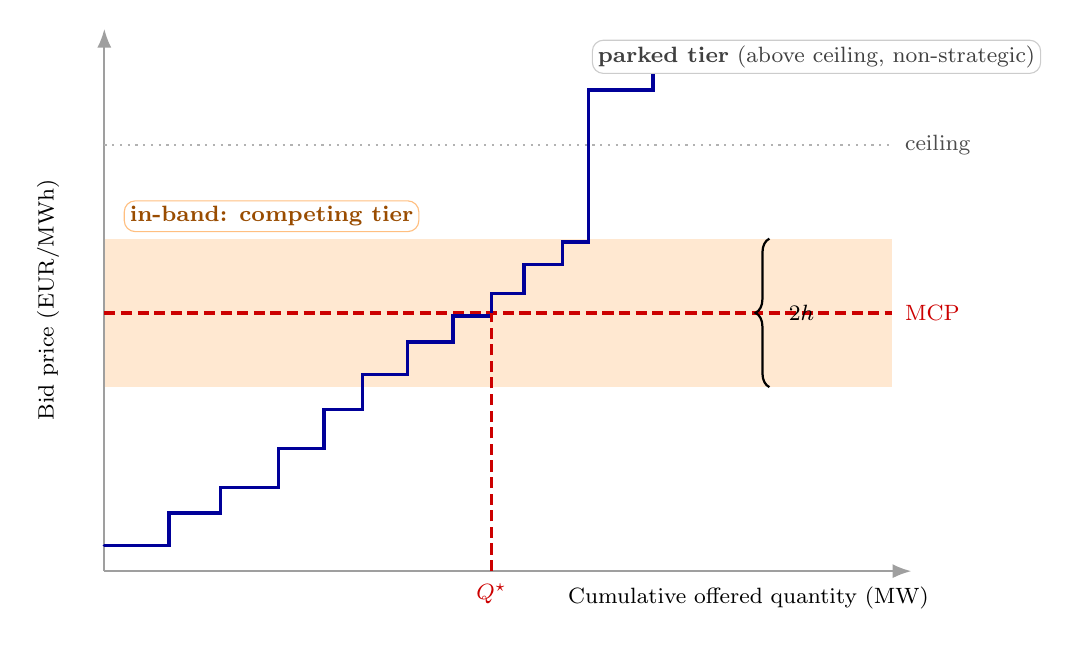
\begin{tikzpicture}[scale=0.82, every node/.style={font=\footnotesize}]
  \def\xmax{12.5}
  \def\ymax{8.4}
  \def\mcp{4}
  \def\h{1.15}
  \def\ceiling{6.6}

  % In-band shaded band ----------------------------------------------------
  \fill[orange!18] (0, \mcp-\h) rectangle (\xmax-0.3, \mcp+\h);

  % Axes -------------------------------------------------------------------
  \draw[-{Latex[length=2.4mm]}, thick, gray!75] (0,0) -- (\xmax,0)
    node[below left=2pt and -10pt, black] {Cumulative offered quantity (MW)};
  \draw[-{Latex[length=2.4mm]}, thick, gray!75] (0,0) -- (0,\ymax);
  \node[rotate=90, anchor=south, black] at (-0.55, \ymax/2)
    {Bid price (EUR/MWh)};

  % Reference horizontal lines --------------------------------------------
  \draw[red!80!black, very thick, dash pattern=on 4pt off 2pt]
    (0, \mcp) -- (\xmax-0.3, \mcp);
  \node[red!80!black, anchor=west] at (\xmax-0.25, \mcp) {MCP};
  \draw[gray!60, dotted, thick] (0, \ceiling) -- (\xmax-0.3, \ceiling);
  \node[gray!60!black, anchor=west] at (\xmax-0.25, \ceiling) {ceiling};

  % Supply step function (sell bids ordered cheapest-to-most-expensive) ---
  \draw[blue!60!black, very thick, line cap=round]
       (0,    0.4) -- (1.0,  0.4)
    -- (1.0,  0.9) -- (1.8,  0.9)
    -- (1.8,  1.3) -- (2.7,  1.3)
    -- (2.7,  1.9) -- (3.4,  1.9)
    -- (3.4,  2.5) -- (4.0,  2.5)
    -- (4.0,  3.05)-- (4.7,  3.05)
    -- (4.7,  3.55)-- (5.4,  3.55)   % low edge of competing tier (in-band)
    -- (5.4,  3.95)-- (6.0,  3.95)   % in-band, just below MCP
    -- (6.0,  4.30)-- (6.5,  4.30)   % in-band, just above MCP
    -- (6.5,  4.75)-- (7.1,  4.75)   % in-band upper
    -- (7.1,  5.10)-- (7.5,  5.10)   % top of competing
    -- (7.5,  7.45)-- (8.5,  7.45)   % parked tier jump (above ceiling)
    -- (8.5,  7.75)-- (10.0, 7.75);

  % Demand vertical (sets MCP at supply crossing) -------------------------
  \draw[red!80!black, very thick, dash pattern=on 4pt off 2pt]
    (6.0, 0) -- (6.0, \mcp);
  \node[red!80!black, below] at (6.0, -0.05) {$Q^\star$};

  % Bandwidth bracket on the right -----------------------------------------
  \draw[decorate, decoration={brace, amplitude=5pt, mirror},
        thick] (\xmax-2.2, \mcp+\h) -- (\xmax-2.2, \mcp-\h);
  \node[anchor=west] at (\xmax-2.05, \mcp) {$2h$};

  % Labels -----------------------------------------------------------------
  \node[orange!60!black, anchor=south west, fill=white, rounded corners,
        inner sep=2pt, draw=orange!50, line width=0.4pt]
    at (0.3, \mcp+\h+0.10) {\textbf{in-band: competing tier}};
  \node[gray!50!black, anchor=south west, fill=white, rounded corners,
        inner sep=2pt, draw=gray!40, line width=0.4pt]
    at (7.55, \ceiling+1.1) {\textbf{parked tier} (above ceiling, non-strategic)};

\end{tikzpicture}
\caption{\textbf{Bandwidth $h$ and the in-band region.} The supply curve
is the sorted sell-bid ladder for one quarter and one market. The market
clears where supply meets demand, fixing the MCP. Bid-shape outcomes
($\sigma_p$, $N_{\text{eff}}$) are computed only on tranches in the
in-band region $[\text{MCP}-h,\ \text{MCP}+h]$ --- the competing tier
where strategic action lives. The parked tier above the clearing-price
ceiling is a non-strategic placeholder (\hyperref[sec:context]{Appendix~C}) and
is excluded by construction.}
\label{fig:in-band-bandwidth}
\end{figure}

Now define the in-band set, MW weights, and in-band weighted mean bid price:
\[
\mathcal{B}_{u,d,p} \;=\; \{k:\,|p_k-\text{MCP}_{d,p}|\le h\}, \qquad w_k \;=\; \frac{\Delta q_k}{\sum_{j\in\mathcal{B}_{u,d,p}} \Delta q_j}, \qquad \bar p_{u,d,p} \;=\; \sum_{k\in\mathcal{B}} w_k\,p_k.
\]

\textbf{Per-curve} (in-band, MW-weighted; one value per (unit, date, period)):
\[
\sigma_{p,\,u,d,p} \;=\; \sqrt{\sum_{k\in\mathcal{B}_{u,d,p}} w_k\,(p_k-\bar p_{u,d,p})^2}, \qquad
N_{\text{eff},\,u,d,p} \;=\; \Big(\sum_{k\in\mathcal{B}_{u,d,p}} w_k^2\Big)^{-1}.
\]
$\sigma_p$ = price spread of the bid ladder within a single quarter; $N_{\text{eff}}$ = effective tranche count of that quarter (1 = a single block, large = many equal-sized tranches).
\vspace{10pt}


\textbf{Aggregate}: $\text{MCP}_{d,p}$ is the OMIE clearing price (EUR/MWh); $Q_{d,p}=\sum_{u,k} q^{\text{cleared}}_{u,d,p,k}$ is the system DA cleared quantity per (date, period)\footnote{The OMIE assigned-power field is per-period instantaneous power (MW), invariant to period length, so one 15-min quarter and one 60-min hour at the same MW are directly comparable as rates. Aggregating MW across the four quarters of a clock-hour gives the stock of energy delivered in that clock-hour, $\text{MWh}_h = \sum_{q\in h}\text{MW}_q\,\Delta t_q$. Aggregate-quantity coefficients below are reported as MWh per clock-hour (numerically equal to the per-period mean MW because the integration is over 1 h, but the unit is energy, not power).}.
\vspace{10pt}

\textbf{In-band quantity primitive.} For each (unit $u$, date $d$, period $p$, IDA session $s$ when applicable) curve, the in-band MW is
\[
m_{u,d,p[,s]} \;=\; \sum_{k\in\mathcal{B}_{u,d,p[,s]}} \Delta q_k,
\]
the total tranche MW falling in the $\pm h$ band around the MCP of that curve. The two quantity outcomes below are both built from $m$.
\vspace{6pt}

\textbf{Within-hour dispersion} (post-only, used to calibrate the critical/flat partition in \hyperref[sec:partition]{\S~2}): for a clock-hour with four quarters $q=1,\dots,4$ post-MTU15, let $\bar{m}=\tfrac{1}{4}\sum_q m_q$ (averaging the per-quarter $m$ values). For each (unit, date, clock-hour) we compute the standard deviation across the four quarters of the clock-hour for each of the five outcomes\footnote{We ommit the $u,h$ subscripts for readability.}:
\[
\begin{aligned}
D_{\text{price}} &= \mathrm{sd}_q(\bar p_q), &
D_{\text{qty}}   &= \mathrm{sd}_q(m_q)/\overline{m}, &
\text{SD}_{\text{price}} &= \mathrm{sd}_q(\text{MCP}_q), \\
D_\sigma &= \mathrm{sd}_q(\sigma_{p,q}), &
D_N      &= \mathrm{sd}_q(N_{\text{eff},q}).
\end{aligned}
\]
$D_{\text{price}}$, $D_{\text{qty}}$, $\text{SD}_{\text{price}}$ are across-quarter shifts in bid \textsc{level}, bid \textsc{volume}, and system clearing prices; $D_\sigma$, $D_N$ are across-quarter shifts in ladder \textsc{spread} and \textsc{tranche count}. All five are zero under the MTU60-equivalent strategy (identical bids in every quarter), so any positive value post-MTU15 is a direct trace of within-hour discrimination.
\vspace{6pt}

\textbf{In-band offered energy (aggregate, per (date, market, tech, hour-class)).} The same primitive $m_{u,d,p[,s]}$ aggregated across tranches (already inside $m$), units of tech $t$, periods $p$ inside an hour, hours $h$ in a class $\mathcal{X}$, and IDA sessions $s$ when applicable, then converted to energy and normalised by class size:
\[
E^{\text{band}}_{t,m,d,\mathcal{X}} \;=\; \frac{1}{|\mathcal{X}|}\sum_{h\in\mathcal{X}}\;\sum_{p\in h}\;\sum_{u\in t,[s]} m_{u,d,p[,s]} \cdot \tau_p,
\]
where $\tau_p$ is the period length in hours ($1$ pre-MTU15, $1/4$ post-MTU15). The $m\cdot\tau_p$ product converts MW to MWh, making the sum invariant to the period count (MTU15 quadrupling does not inflate it mechanically). The $1/|\mathcal{X}|$ normalisation expresses the result as MWh per class-hour, directly comparable across classes of different sizes. (Note that $D_{\text{qty}}$ above is already a cross-window-comparable normalised quantity --- a coefficient of variation in $m$ across the four quarters --- so it needs no further rescaling; $E^{\text{band}}$ needs both $\tau_p$ and $|\mathcal{X}|$ to be cross-window comparable because it sums rather than ratios.)
\vspace{6pt}

\textbf{Cross-market wedge.} Per-clock-hour day-ahead/intraday price gap and its within-day spread:
\[
\Delta_{d,h} \;=\; \text{MCP}^{\text{DA}}_{d,h} - \text{MCP}^{\text{IDA}}_{d,h}, \qquad
\Delta^{\text{SD}}_d \;=\; \mathrm{sd}_h(\Delta_{d,h}).
\]
$\Delta_{d,h}$ is cross-market disagreement at clock-hour $h$; $\Delta^{\text{SD}}_d$ is how much that disagreement varies across the 24 clock-hours of day $d$. Both $\text{MCP}^{\text{DA}}_{d,h}$ and $\text{MCP}^{\text{IDA}}_{d,h}$ are computed at the clock-hour level by averaging \emph{within each market} over whatever sub-hour structure that market has on date $d$\footnote{Not sure about this, maybe I should exploit all the granularity!}: DA collapses the four 15-min quarters post-DA15 (one observation pre-DA15); IDA collapses the three auction sessions and (post-ID15) the four within-hour quarters. The wedge then compares two equally-aggregated clock-hour means and is therefore directly comparable across regimes: it does not mechanically widen just because IDA gains a quarter dimension. Under asymmetric granularity (ID15: DA 60-min, IDA 15-min), each clock-hour hosts four IDA quarter-prices against a single DA price, so $\Delta_{d,h}$ can move further where within-hour residual demand actually varies --- this is a behavioural channel, not a mechanical one.

\paragraph{Seasonality.} Spanish electricity has strong intra-year seasonality. It bites on the level outcomes --- clearing prices and per-tech cleared energy --- which co-move with heating demand in winter, cooling demand in summer, and the hydrological cycle. Bid-shape outcomes ($\sigma_p$, $N_{\text{eff}}$) are MCP-centered and MW-weighted on the in-band ladder, so price-level seasonality does not transmit.
\vspace{6pt}

\section*{2. The critical/flat partition: where granular pricing has economic content}
\addcontentsline{toc}{section}{2. The critical/flat partition: where granular pricing has economic content}
\phantomsection\label{sec:partition}

\paragraph{Intuition.} Granular pricing only has economic content where within-hour residual demand\footnote{Spanish-market convention calls this the \emph{hueco t\'ermico} (thermal gap) --- the load that thermal and other dispatchable generation must cover after subtracting wind and solar.} actually varies; if a clock-hour is internally flat, the four quarters look the same and there is nothing to discriminate on. We measure within-hour variation by $\sigma_{\text{within}}(h,d) = \mathrm{sd}_q[\text{load}-\text{wind}-\text{solar}]_{q,h,d}$ on 15-min residual-demand data\footnote{ENTSO-E Transparency Platform: A65 (actual total load) and the wind/solar component of A75 (actual generation per type, PSR codes B16, B18, B19); window 2023-01-01 to 2026-05-14.} and partition clock-hours by median $\sigma_{\text{within}}$:
\begin{itemize}\setlength{\itemsep}{1pt}
\item \textbf{Critical} $\mathcal{C}=\mathcal{C}_M\cup\mathcal{C}_E$ with $\mathcal{C}_M=\{5,\dots,8\}$ (\emph{morning ramp}) and $\mathcal{C}_E=\{16,\dots,22\}$ (\emph{evening ramp}); $\sigma_{\text{within}}\in[522,1303]$ MW overall. The two sub-classes have different seasonal patterns (sunrise/sunset timing shifts the start of solar generation across the class boundaries), and bid-side analyses below treat them separately so each sub-class's seasonality is modelled on its own pattern.
\item \textbf{Flat} $\mathcal{F}=\{1,2,3\}$: overnight; $\sigma_{\text{within}}\in[336,357]$ MW.
\item \textbf{Midday} $\{11,\dots,14\}$ (solar-marginal, $\sigma_{\text{within}}\in[468,502]$ MW): excluded from main specs; kept for falsification (\hyperref[sec:5a]{Appendix~A.2}).
\end{itemize}

\paragraph{Formal calibration of the partition (post-only).} Let $D_{d,h}$ stand for any one of the five within-hour dispersion outcomes ($D_{\text{price}}$, $D_{\text{qty}}$, $\text{SD}_{\text{price}}$, $D_\sigma$, $D_N$) on date $d$, clock-hour $h$. Under MTU60 the within-hour quarter dimension does not exist, so $D_{d,h}$ is mechanically zero pre-reform; we use the post-MTU15 sample to \emph{describe} where within-hour dispersion lives across hour-classes. A date-FE regression is a convenient way to summarise the critical$-$flat differential:
\[
D_{d,h} \;=\; \delta_d \;+\; \theta\,\mathbf{1}\{h\in\mathcal{C}\} \;+\; \varepsilon,
\]
fit per outcome. $\theta$ is the post-MTU15 critical$-$flat dispersion gap. This is a \textbf{descriptive contrast, not a causal estimate}.

\begin{center}
\footnotesize
\setlength{\tabcolsep}{6pt}
\begin{tabular}{l l c c c}
\toprule
\textbf{Outcome} & \textbf{Subsample} & \textbf{ID15} & \textbf{DA15} & \textbf{crit/flat ratio (IDA, DA)} \\
\midrule
$D_{\text{price}}$ (EUR/MWh)         & per unit (pooled) & $0.39^{***}$ (0.05)    & $1.35^{***}$ (0.11)   & $4.1\times,\ 7.4\times$ \\
$D_{\text{qty}}$ (CV)                & per unit (pooled) & $0.024^{***}$ (0.003)  & $0.033^{***}$ (0.002) & $4.3\times,\ 4.9\times$ \\
$\text{SD}_{\text{price}}$ (EUR/MWh) & system            & $4.55^{***}$ (0.40)    & $3.97^{***}$ (0.37)   & $2.8\times,\ 2.6\times$ \\
\addlinespace
$D_\sigma$ (EUR/MWh)                 & CCGT       & $-0.24$ (0.35)         & $0.57^{***}$ (0.10)    & --,\ $5.9\times$ \\
                                     & Hydro      & $0.48^{***}$ (0.07)    & $1.22^{***}$ (0.16)    & $2.2\times,\ 3.1\times$ \\
                                     & Hydro pump & $0.16^{***}$ (0.03)    & $0.66^{***}$ (0.15)    & $3.7\times,\ 10.6\times$ \\
                                     & Wind       & $-0.003$ (0.005)       & $0.04^{***}$ (0.02)    & $1.0\times,\ 2.3\times$ \\
\bottomrule
\end{tabular}
\captionof{table}{\textbf{Post-MTU15 critical$-$flat within-hour dispersion gap, by outcome.} \textit{SE clustered by date}; $^{***}p<0.01$. Bid-level rows ($D_{\text{price}}$, $D_{\text{qty}}$, $\text{SD}_{\text{price}}$) are bandwidth-free. The per-tech $D_\sigma$ rows are computed at the new $p_{90}$ baseline (\hyperref[sec:setup]{\S~1}): ID15 column uses post-ID15 IDA data with $h{=}62$; DA15 column uses post-DA15 DA data with $h{=}50$. \emph{Reading.} Under DA15, $D_\sigma$ is positive and significant for all three dispatchable techs in DA --- CCGT $0.57$, hydro $1.22$, pump-storage $0.66$ --- with the largest critical/flat ratio for CCGT ($5.9\times$). Under ID15, hydro and pump-storage widen their IDA within-hour ladders ($0.48$ and $0.16$), while CCGT IDA $D_\sigma$ is not distinguishable from zero --- consistent with combined-cycle gas mostly competing in DA rather than IDA at this stage. Wind stays small everywhere, consistent with its operational, uniform-across-hour-classes engagement (\hyperref[sec:4-c-id15-ida]{\S~4.C.2}).}
\end{center}

\section*{3. Identification: DiD for bid shape, BSTS for prices and quantities}
\addcontentsline{toc}{section}{3. Identification: DiD for bid shape, BSTS for prices and quantities}
\phantomsection\label{sec:identification}

$u$ unit; $d$ date; $p$ period; $h$ clock-hour; $s$ IDA session; $T_r$ reform date. Treatment status $D_{d,h} \equiv \mathbf{1}\{d\ge T_r\}\cdot\mathbf{1}\{h\in\mathcal{C}\}$; sample restricted to $h\in\mathcal{C}\cup\mathcal{F}$ for the DiD.

\subsection*{3.A. Spec A: Bayesian Structural Time Series for prices, cleared energy, and wedge SD}\addcontentsline{toc}{subsection}{3.A. Spec A: BSTS for prices, cleared energy, and wedge SD}\phantomsection\label{sec:bsts}

\emph{Idea.} A Bayesian Structural Time Series (BSTS) model \citep{brodersen_2015}, as applied to the EPEX 15-min reform by \citet{markle_huss_2017}, fits a flexible state-space decomposition of the response on the pre-reform window and extrapolates forward to construct a counterfactual: what the outcome \emph{would} have looked like in the post-window absent the reform. The treatment effect is the gap between observed and counterfactual. The strength over other methods is that BSTS handles complex seasonality and trend \emph{internally}, useful here since the pre-windows are short.

\emph{Model.} The daily response decomposes additively into trend, weekly cycle, exogenous covariates, and noise:
\[
y_t \;=\; \underbrace{\mu_t}_{\text{trend}} \;+\; \underbrace{\gamma_t}_{\text{weekly cycle}} \;+\; \underbrace{X_t'\beta}_{\text{exogenous covariates}} \;+\; \underbrace{\varepsilon_t}_{\text{noise}}.
\]
$\mu_t$ is a random walk with stochastic slope (a slowly evolving local level), $\gamma_t$ a 7-day cycle, and $X_t = (\text{wind GWh}, \text{solar GWh}, \text{gas price EUR})$ exogenous covariates that absorb merit-order shifts driven by renewable supply and fuel prices (a spike-and-slab prior on $\beta$ shrinks unused regressors). Demand is excluded to avoid simultaneity.

\emph{Outcomes $y_t$.} DA or IDA daily-average clearing prices, per-tech daily cleared GWh, within-day wedge SD $\Delta^{\text{SD}}_d$ overall and per hour-class $\Delta^{\text{SD},\mathcal{X}}_d = \mathrm{sd}_{h\in\mathcal{X}}(\Delta_{d,h})$ for $\mathcal{X}\in\{\mathcal{C}_M, \mathcal{C}_E, \mathcal{M},\mathcal{F}\}$.

\emph{Estimand.} Conditional on $X_t$, the post-cutover counterfactual equals the pre-trained extrapolation $\hat y_t(0)$. The average treatment effect on the post-window is
\[
\bar\tau \;=\; \tfrac{1}{|\text{post}|}\textstyle\sum_{t\ge T_r}\bigl(y_t - \hat y_t(0)\bigr),
\]
reported together with its 95\% credible interval from the MCMC posterior produced by the \texttt{CausalImpact} R package.

\emph{Windows} hold the relevant regulatory regime constant across pre and post (Figure~\ref{fig:bsts-windows}): DA15 pre starts at the reforzada onset; ID15 pre starts at the post-IDA-reform 3-session architecture and stops at the blackout.

\begin{figure}[H]
\centering
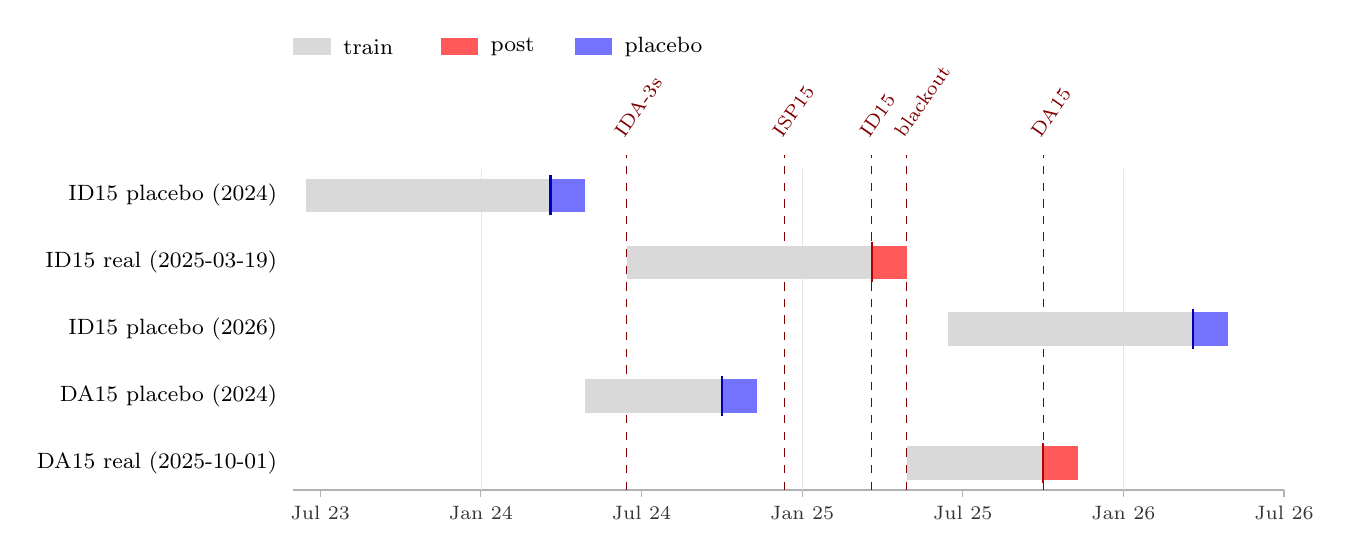
\begin{tikzpicture}[scale=0.85, every node/.style={font=\footnotesize}]
  % x-axis: months from 2023-06 (=0) to 2026-07 (=37). 0.4 cm per month.
  \def\xs{0.40}
  % Row y-positions (5 rows)
  \def\yIDpA{4.4} \def\yIDr{3.4} \def\yIDpB{2.4} \def\yDAp{1.4} \def\yDAr{0.4}
  \def\hbar{0.25}

  % Axis line
  \draw[gray!60, thick] (0,0) -- (\xs*37,0);
  % Half-year ticks with month-year labels
  \foreach \m/\lbl in {1/{Jul 23}, 7/{Jan 24}, 13/{Jul 24}, 19/{Jan 25}, 25/{Jul 25}, 31/{Jan 26}, 37/{Jul 26}} {
    \draw[gray!60] (\xs*\m, 0) -- (\xs*\m, -0.1);
    \node[anchor=north, gray!40!black, font=\scriptsize] at (\xs*\m, -0.1) {\lbl};
  }
  % Light vertical guides at January of each year
  \foreach \m in {7, 19, 31} {
    \draw[gray!20, very thin] (\xs*\m, 0) -- (\xs*\m, 4.8);
  }
  % Reform vertical lines (dashed, with rotated short-label tags at top)
  \foreach \m/\lbl in {12.45/{IDA-3s},
                       18.35/{ISP15},
                       21.6/{ID15},
                       22.9/{blackout},
                       28.0/{DA15}} {
    \draw[red!50!black, dashed, thin] (\xs*\m, 0) -- (\xs*\m, 5.0);
    \node[anchor=south west, red!50!black, font=\scriptsize, rotate=55]
      at (\xs*\m, 5.05) {\lbl};
  }

  % ID15 placebo 2024: pre 2023-06-14 (0.45) -> 2024-03-18 (9.6); post 9.6 -> 10.9
  \fill[gray!30] (\xs*0.45,\yIDpA-\hbar) rectangle (\xs*9.6,\yIDpA+\hbar);
  \fill[blue!55] (\xs*9.6,\yIDpA-\hbar) rectangle (\xs*10.9,\yIDpA+\hbar);
  \draw[blue!70!black, thick] (\xs*9.6,\yIDpA-\hbar-0.05) -- (\xs*9.6,\yIDpA+\hbar+0.05);
  \node[anchor=east] at (-0.1, \yIDpA) {ID15 placebo (2024)};

  % ID15 real: pre 2024-06-14 (12.45) -> 2025-03-18 (21.6); post 21.6 -> 22.9
  \fill[gray!30] (\xs*12.45,\yIDr-\hbar) rectangle (\xs*21.6,\yIDr+\hbar);
  \fill[red!65] (\xs*21.6,\yIDr-\hbar) rectangle (\xs*22.9,\yIDr+\hbar);
  \draw[red!70!black, thick] (\xs*21.6,\yIDr-\hbar-0.05) -- (\xs*21.6,\yIDr+\hbar+0.05);
  \node[anchor=east] at (-0.1, \yIDr) {ID15 real (2025-03-19)};

  % ID15 placebo 2026: pre 2025-06-14 (24.45) -> 2026-03-18 (33.6); post 33.6 -> 34.9
  \fill[gray!30] (\xs*24.45,\yIDpB-\hbar) rectangle (\xs*33.6,\yIDpB+\hbar);
  \fill[blue!55] (\xs*33.6,\yIDpB-\hbar) rectangle (\xs*34.9,\yIDpB+\hbar);
  \draw[blue!70!black, thick] (\xs*33.6,\yIDpB-\hbar-0.05) -- (\xs*33.6,\yIDpB+\hbar+0.05);
  \node[anchor=east] at (-0.1, \yIDpB) {ID15 placebo (2026)};

  % DA15 placebo: pre 2024-04-28 (10.9) -> 2024-09-30 (16.0); post 16.0 -> 17.3
  \fill[gray!30] (\xs*10.9,\yDAp-\hbar) rectangle (\xs*16.0,\yDAp+\hbar);
  \fill[blue!55] (\xs*16.0,\yDAp-\hbar) rectangle (\xs*17.3,\yDAp+\hbar);
  \draw[blue!70!black, thick] (\xs*16.0,\yDAp-\hbar-0.05) -- (\xs*16.0,\yDAp+\hbar+0.05);
  \node[anchor=east] at (-0.1, \yDAp) {DA15 placebo (2024)};

  % DA15 real: pre 2025-04-28 (22.9) -> 2025-09-30 (28.0); post 28.0 -> 29.3
  \fill[gray!30] (\xs*22.9,\yDAr-\hbar) rectangle (\xs*28.0,\yDAr+\hbar);
  \fill[red!65] (\xs*28.0,\yDAr-\hbar) rectangle (\xs*29.3,\yDAr+\hbar);
  \draw[red!70!black, thick] (\xs*28.0,\yDAr-\hbar-0.05) -- (\xs*28.0,\yDAr+\hbar+0.05);
  \node[anchor=east] at (-0.1, \yDAr) {DA15 real (2025-10-01)};

  % Legend (above reform labels)
  \fill[gray!30] (\xs*0, 6.5) rectangle (\xs*1.4, 6.75);
  \node[anchor=west] at (\xs*1.5, 6.62) {train};
  \fill[red!65] (\xs*5.5, 6.5) rectangle (\xs*6.9, 6.75);
  \node[anchor=west] at (\xs*7.0, 6.62) {post};
  \fill[blue!55] (\xs*10.5, 6.5) rectangle (\xs*11.9, 6.75);
  \node[anchor=west] at (\xs*12.0, 6.62) {placebo};
\end{tikzpicture}
\captionof{figure}{\textbf{Spec~A windows.} Each row is one BSTS run. Grey: pre-window (model training). Red: post-window after the real reform cutover. Blue: post-window after a same-calendar placebo cutover (one year before or after the real reform). Pre-windows are restricted so that the relevant regulatory regime is held constant across pre and post: DA15 pre starts at the reforzada onset (2025-04-28); ID15 pre starts at the post-IDA-reform 3-session architecture (2024-06-14) and stops at the blackout (2025-04-28). The independent 2026 placebo for ID15 doubles the falsifier --- a calendar-symmetric counterpart on the other side of the real reform.}
\label{fig:bsts-windows}
\end{figure}

\emph{Placebo cross-check and the joint 95\% credible interval.} The same BSTS is re-run on a same-calendar window one year before each reform with a fake cutover. This gives a \emph{placebo posterior}: what BSTS attributes to that date in a year with no reform. Two cases:
\begin{itemize}\setlength{\itemsep}{1pt}
\item \emph{Real significant, placebo near zero}: the effect is reform-attributable.
\item \emph{Real and placebo both significant and similar in magnitude}: BSTS is picking up a recurring calendar shift its seasonality model does not fully absorb, and the ``real'' estimate is not separable from that shift.
\end{itemize}
A sharp filter is the \emph{joint 95\% credible interval}: treating real and placebo posteriors as independent, the difference $\bar\tau_{\text{real}} - \bar\tau_{\text{placebo}}$ has variance $\sigma^2_{\text{real}} + \sigma^2_{\text{placebo}}$, and a 95\% interval excluding zero rejects the recurring-calendar story. Reform attribution requires (i) a significant real-window estimate \emph{and} (ii) the placebo not running in the same direction with similar magnitude; the joint interval is reported as a check.

\emph{Drift diagnostic: near-window vs.\ full-window estimate.}\phantomsection\label{sec:drift-diagnostic} A characteristic signature of BSTS counterfactual error is an effect that emerges only in the late segment of the post-window: the observed series tracks the counterfactual closely for the first weeks after the cutover and then diverges as the pre-trained extrapolation drifts away from the realised series. We diagnose this by re-running BSTS with a near-cutover post-window (14 days instead of 40); a genuine reform response is similar in sign and magnitude at both window lengths, while drift collapses the near-window estimate toward zero.

\subsection*{3.B. Spec B: per-hour-class BSTS on bid-level outcomes}\addcontentsline{toc}{subsection}{3.B. Spec B: per-hour-class BSTS on bid-level outcomes}\phantomsection\label{sec:smart_desc}
To identify within-day reallocation in bid \emph{levels}, the same Spec~A BSTS is run \emph{independently} on each (tech, market, hour-class) cell for two bid-level outcomes:
\begin{itemize}\setlength{\itemsep}{1pt}
  \item $\bar p_{t,m,h,d}$: MW-weighted mean of in-band tranche prices.
  \item $E^{\text{band}}_{t,m,d,\mathcal{X}}$: in-band offered energy in MWh per class-hour (\hyperref[sec:setup]{\S~1}). The $\tau_p$ factor makes the post-MTU15 quarter-sum invariant to the period count; the $1/|\mathcal{X}|$ normalisation makes the levels comparable across hour-classes of different sizes.
\end{itemize}
The readable summary is the real-window posterior \emph{and the same-calendar 2024 placebo posterior reported side by side for each hour-class separately} (\hyperref[tab:specB-id15]{Tables}), not the (critical $-$ flat) differential, which would collapse information when two hour-classes move in the same direction at different magnitudes. For each (tech, market, outcome, hour-class) we form $\bar\tau_{\text{real}} - \bar\tau_{\text{placebo}}$ from two BSTS posteriors (real and placebo) that are independent across years, and use the same joint 95\% credible-interval reading as in \hyperref[sec:bsts]{\S~3.A}\footnote{Note that there is huge within day dependance, so this is not a big issue that shrinks prediction intervals at a huge cost.}. We avoid per-(single-hour) BSTS because at that resolution residual noise dominates the seasonal signal.

\subsection*{3.C. Spec C: per-curve DiD for bid shape}\addcontentsline{toc}{subsection}{3.C. Spec C: per-curve DiD for bid shape}\phantomsection\label{sec:did}
For per-tech bid-shape outcomes $Y\in\{\sigma_p, N_{\text{eff}}\}$ we use the DiD:
\[
Y_{u,d,p[,s]} = \alpha_u + \beta\,\mathbf{1}\{d\ge T_r\} + \xi\,\mathbf{1}\{h\in\mathcal{C}\} + \theta\,D_{d,h} + \varepsilon, \qquad \text{SEs clustered by date.}
\]
The justification is mechanism-based. \textbf{The granularity reform's bid-shape effect is structurally a critical-hours effect.} Differentiated bidding only pays off where the residual demand curve is steep enough to reward it: in critical hours that condition holds, so $4$ quarter-prices instead of $1$ unlock real price discrimination; in flat hours the curve is shallow and the extra granularity is mostly wasted optionality. The (critical $-$ flat) differential $\theta$ therefore IS the granularity-enabled discrimination, not a residual we are netting out. Flat hours act as a low-exposure within-day control --- not a zero-exposure one, since MTU15 reaches them too.

For the level outcomes --- prices and cleared MW in \hyperref[sec:bsts]{\S~3.A}, in-band offered energy per hour-class in \hyperref[sec:smart_desc]{\S~3.B} --- we keep BSTS: per-hour-class BSTS already lets the data reveal any critical-hour concentration as heterogeneity across the four estimates, without imposing the critical-flat differential as the identifying restriction.

Since each MTU15 reform is studied separately, this is a standard $2\times 2$ DiD without staggered-treatment negative weights \citep[ch.~3]{de_chaisemartin_2026}.

\subsection*{3.D. \textcolor{red}{Ongoing extension:} BSTS-style counterfactual for the full bid curve}
\addcontentsline{toc}{subsection}{3.D. Ongoing extension: BSTS-style counterfactual for the full bid curve}\phantomsection\label{sec:fbr}
A natural generalisation of Spec~B is to replace the scalar in-band summaries ($\bar p$ and $E^{\text{band}}$) with the \emph{full submitted-bid step function} --- treat each daily aggregate supply curve as a functional observation and predict its post-reform counterfactual in the same BSTS spirit.

The motivation is methodological. Modelling seasonality on the full curve is more natural than modelling it on the scalar summaries: both $\bar p$ and $E^{\text{band}}$ are MCP-relative (the band slides with MCP, and MCP itself has strong seasonality), whereas the supply curve $S(p)$ is defined on the same price domain every day, so weather and fundamentals can be regressed pointwise on $p$ without the band moving underneath the outcome.

We are exploring this via functional factor regression \citep{otto_winter_2025}, which controls for seasonality through hourly weather (wind, solar) as functional regressors plus daily gas as a scalar regressor --- the same identifying logic as Spec~A but on the entire curve rather than on a scalar outcome. The output is a curve-level placebo-net shift $\Delta S(p)$: the gap, at each bid price $p$, between the post-reform supply curve and the counterfactual the model would have predicted absent the reform. Results are preliminary and not reported here.

\vspace{10pt}

\section*{4. Results: bid-shape widening, day-ahead CCGT auction-cleared scale-up, and directional price movements}
\addcontentsline{toc}{section}{4. Results: bid-shape widening, day-ahead CCGT auction-cleared scale-up, and directional price movements}
\phantomsection\label{sec:results}

\noindent Findings are organised one spec at a time. All three specs share the same wind+solar+gas covariates and the 2024 same-calendar placebo.

\subsection*{4.A. Spec A: prices and per-tech cleared energy}
\addcontentsline{toc}{subsection}{4.A. Spec A: prices and per-tech cleared energy}\phantomsection\label{sec:4-specA}
\begin{center}
\footnotesize
\setlength{\tabcolsep}{4pt}
\begin{tabular}{l l r r r r r r}
\toprule
                & & \multicolumn{3}{c}{\textbf{ID15}} & \multicolumn{3}{c}{\textbf{DA15}} \\
\cmidrule(lr){3-5} \cmidrule(lr){6-8}
\textbf{Outcome} & \textbf{Tech} & Real & Placebo & Net & Real & Placebo & Net \\
\midrule
DA clearing price (EUR/MWh)  & ---        & $-38.39^{***}$ & $-13.71$       & $-24.68$         & $2.97$         & $-8.54$         & $11.51$ \\
IDA clearing price (EUR/MWh) & ---        & $-38.34^{***}$ & $-18.08^{*}$   & $-20.26$         & $5.13$         & $-6.55$         & $11.68$ \\
\addlinespace
DA cleared (GWh/day)         & CCGT       & $10.48$        & $-10.83$       & $21.31$          & $40.31^{***}$  & $-18.69^{***}$  & $58.99^{***}$ \\
                             & Hydro      & $-4.36$        & $15.71^{***}$  & $-20.07^{**}$    & $6.16^{*}$     & $9.28^{***}$    & $-3.12$ \\
                             & Hydro pump & $-0.82$        & $-0.30$        & $-0.52$          & $4.43^{***}$   & $1.42^{*}$      & $3.02^{*}$ \\
                             & Wind       & $9.64^{*}$     & $9.54^{*}$     & $0.10$           & $13.16^{***}$  & $2.15$          & $11.00^{*}$ \\
                             & Solar      & $11.28^{***}$  & $10.53^{***}$  & $0.74$           & $-3.37$        & $1.38$          & $-4.74$ \\
                             & Nuclear    & $53.69^{**}$   & $-50.45$       & $104.14^{*}$     & $-18.21^{**}$  & $-34.77^{***}$  & $16.56$ \\
\addlinespace
IDA cleared (GWh/day)        & CCGT       & $-8.08^{***}$  & $-9.18^{***}$  & $1.10$           & $0.68$         & $-2.38$         & $3.06$ \\
                             & Hydro      & $-1.27^{***}$  & $4.98^{***}$   & $-6.25^{***}$    & $-0.41$        & $1.20^{*}$      & $-1.60^{*}$ \\
                             & Hydro pump & $-0.37^{*}$    & $0.54^{**}$    & $-0.91^{**}$     & $0.10$         & $-0.27$         & $0.37$ \\
                             & Wind       & $5.34^{***}$   & $7.99^{***}$   & $-2.65^{**}$     & $-2.63^{***}$  & $2.28^{*}$      & $-4.91^{***}$ \\
                             & Solar      & $6.70^{***}$   & $2.55^{***}$   & $4.16^{***}$     & $-5.86^{***}$  & $-0.34$         & $-5.52^{***}$ \\
                             & Nuclear    & $11.51^{***}$  & $19.06^{***}$  & $-7.56$          & $1.68$         & $-5.43$         & $7.11$ \\
\bottomrule
\end{tabular}
\captionof{table}{\textbf{Spec~A BSTS effects on clearing prices and per-tech cleared energy.} Bayesian posterior point estimates; stars in Real/Placebo cells are tail-probability stars on each individual posterior ($^{*}p{<}0.10$, $^{**}p{<}0.05$, $^{***}p{<}0.01$). The Net column is the placebo-net effect (Real $-$ Placebo) with joint $z$-test stars derived under independent-Gaussian-posterior approximation: $\text{Net}/\sqrt{\text{SE}^2_{\text{real}}+\text{SE}^2_{\text{placebo}}}$. Windows in \hyperref[sec:bsts]{\S~3.A}; placebo columns re-run BSTS on the same calendar window in 2024 with a fake cutover. Observed-vs-counterfactual series in Figures~\ref{fig:bsts-id15}--\ref{fig:bsts-da15}.}
\label{tab:bsts-spec-a}
\end{center}

\begin{figure}[H]
\centering
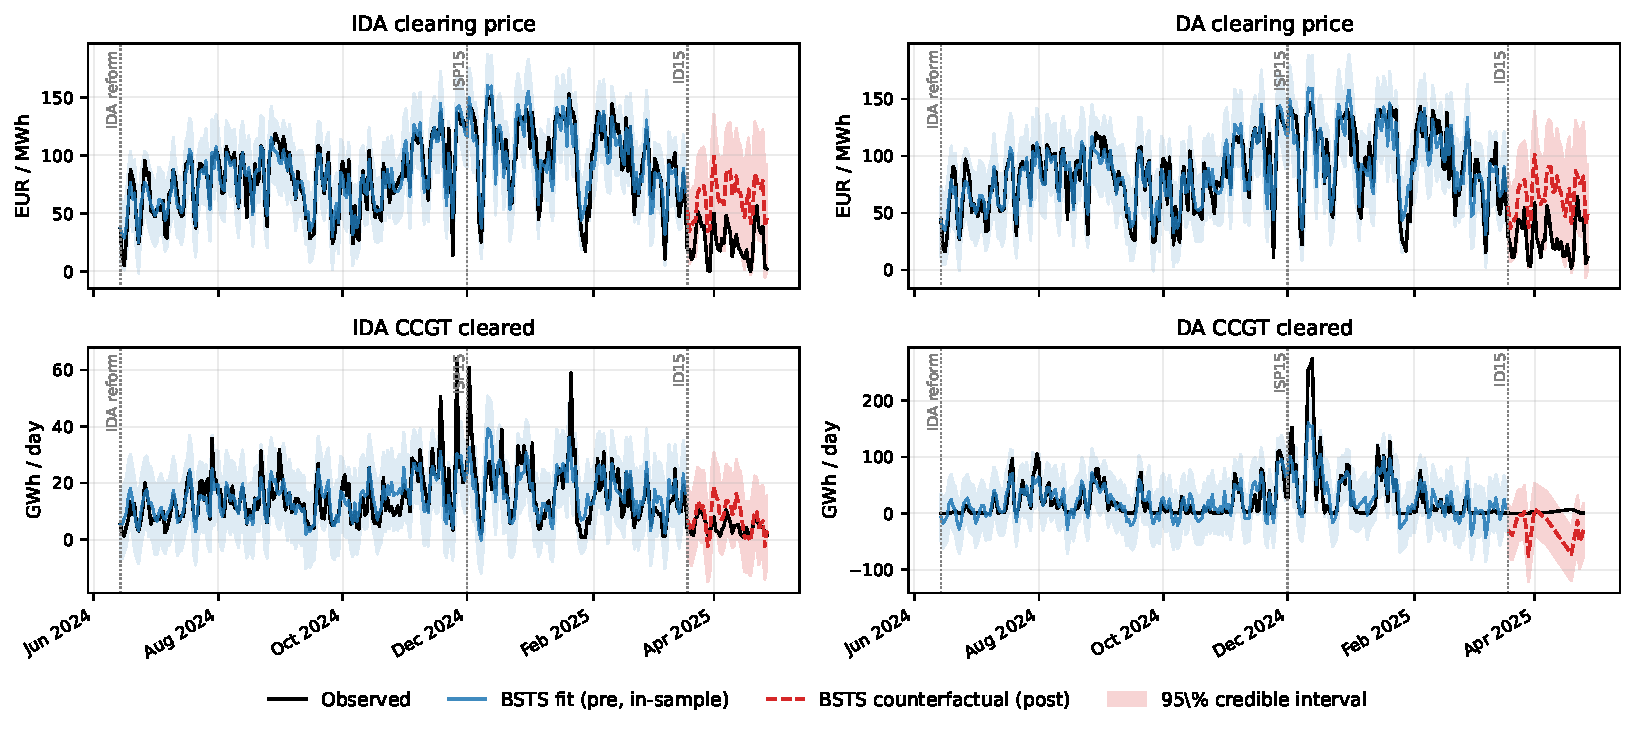
\includegraphics[width=0.9\linewidth]{fig_bsts_id15_effects.pdf}
\caption{\textbf{ID15 effects on both markets} (2$\times$2 zoomed view, 40-day pre-blackout post-window). Black: observed (7-day MA). Blue: BSTS in-sample fit on the pre-window with 95\% band. Red dashed: out-of-sample counterfactual with 95\% band. Cutover 2025-03-19; blackout 2025-04-28. Both IDA and DA clearing prices (top row) drop below the counterfactual by similar magnitudes on the same day, even though ID15 only changed intraday granularity --- the cross-market rational-anticipation channel into day-ahead (finding \hyperref[sec:4ii]{(ii)}).}
\label{fig:bsts-id15}
\end{figure}

\begin{figure}[H]
\centering
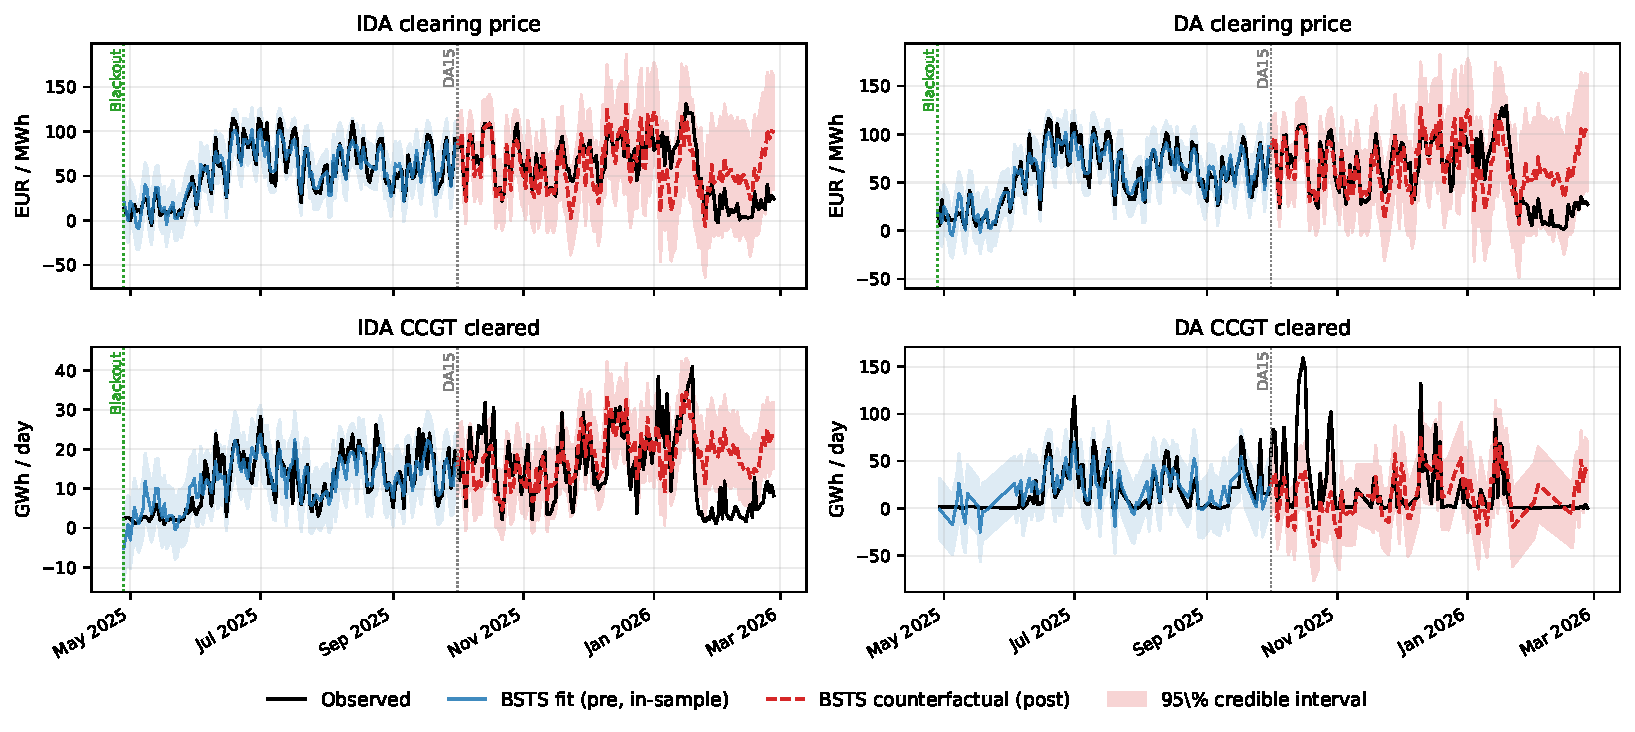
\includegraphics[width=0.9\linewidth]{fig_bsts_da15_effects.pdf}
\caption{\textbf{DA15 effects on both markets} (2$\times$2 zoomed view, post-window through 2026-02-26). Same colour scheme as Figure~\ref{fig:bsts-id15}. Cutover 2025-10-01; reforzada-constant pre-window starts 2025-04-28. The DA CCGT panel (bottom-right) is the one quantity outcome where the observed series visibly departs from the counterfactual post-cutover --- the CCGT scale-up of \hyperref[sec:4iii]{\S~4.A.2}. By contrast, the IDA panels show no backwards transmission (intraday clearing follows day-ahead, so a DA-side reform cannot propagate backwards).}
\label{fig:bsts-da15}
\end{figure}

\subsubsection*{4.A.1. ID15 clearing-price drop in both markets}\phantomsection\label{sec:4ii}
Both DA and IDA clearing prices drop sharply under ID15 (Table above; top row of Figure~\ref{fig:bsts-id15}). The cross-market symmetry is the signature: both markets drop by similar magnitudes on the same day even though ID15 only changed \emph{intraday} granularity --- the rational-anticipation channel into day-ahead. The BSTS conditions on wind, solar, and gas, so the drop is net of the merit-order shift; the pre-window in-sample fit is tight. \emph{Verdict.} The 2024 same-calendar placebo also runs negative; the joint placebo-net 95\% interval brackets zero, so the level effect is not retained. We report the raw drop and its cross-market signature only. DA15 price effects are small and not directional.

\subsubsection*{4.A.2. DA15 day-ahead CCGT cleared scale-up concentrates in critical hours}\phantomsection\label{sec:4iii}
The only level-shift finding to survive the joint 95\% placebo-net test (Figure~\ref{fig:bsts-da15}, bottom-right). MTU15-DA lets combined-cycle gas discriminate finely within the hour, raising its expected acceptance probability across the four quarters of a peak hour --- same channel as the bid-shape widening in \hyperref[sec:4i]{\S~4.C.1}. Running the Spec~A BSTS at hour-class resolution on cleared MWh shows the scale-up concentrates almost entirely in critical hours, with a smaller flat-hour contribution and essentially nothing in midday (where solar saturation displaces gas) --- the granularity-bites-where-within-hour-residual-demand-varies channel made direct. The scale-up is also one-sided across markets: substantial in DA, essentially unchanged in IDA --- CCGT migrates \emph{into} DA without losing its IDA arm in cleared terms. Extending the post-window through winter shrinks but does not flip the estimate. Hydro and nuclear are essentially null.

\emph{Note.} OMIE auction-cleared MW is pre-restriction by construction: the adjustments REE makes through the technical-restrictions process do not enter in these programs\footnote{Programa Diario Base de Casación (PDBC), for DA; and Programa Intradiario Base de Casación Incremental (PIBCI), for IDA.}. The scale-up reported here is therefore a shift in the day-ahead \emph{competitive clearing}, not in REE's restriction call (see \hyperref[sec:context]{Appendix~C}).

However, \textbf{competitive clearing anticipates expected REE's intervention}, so we should flag this\footnote{As illustratiion, check SNC-DE-175-17 CNMC 2019 resolution, in which Naturgy was sanctioned for undercommiting with gas plants in the DA and wait to being called in the technical-restrictions Fase I up market, which is pay-as-bid and usually more profitable (check the descriptive section for a description of the issue).}.

\subsubsection*{4.A.3. Renewable cleared MW reallocates toward the granular market}\phantomsection\label{sec:4-renewable}
Renewables cannot reposition their physical generation --- it follows weather --- but aggregators can reposition where the generation is \emph{offered}. Under DA15, day-ahead cleared MW rises broadly across hour-classes for wind (aggregators push the entire output into DA), while the intraday side falls. Solar reallocates time-of-day rather than only market-side: DA cleared rises in midday (where solar generates) and falls in critical hours; IDA cleared falls across the day. Under ID15, intraday cleared MW rises for solar while day-ahead is unchanged.

\emph{Mechanism.} The same upstream-migration logic as the dispatchable fleet in \hyperref[sec:4iii]{\S~4.A.2} (finer offering raises expected acceptance probability), reinforced by a renewable-specific channel: ISP15 (December 2024) moved REE's imbalance settlement to 15-min, so any intra-hour gap between scheduled and realised generation now triggers a 15-min imbalance penalty. Scheduling into a 60-min market locks the unit into a single hourly schedule even when its 15-min forecast varies within the hour; scheduling into the granular (15-min) market lets the unit submit a schedule that tracks its 15-min forecast and minimises the imbalance bill. Wind and solar have the largest within-hour forecast variance among Spanish techs, so they benefit most from the granular-market shift.

\subsubsection*{4.A.4. ID15 within-day wedge SD jumps in critical hours}\phantomsection\label{sec:4-wedge}
The wedge \emph{level} BSTS is null in both reforms. The within-day wedge SD $\Delta^{\text{SD}}_d$, by contrast, jumps sharply under ID15 and concentrates in critical hours.\footnote{Wedge SD placebo-net under ID15: $2.16$~EUR/MWh (joint 95\% $[0.62, 3.70]$) overall; $3.14$ in critical hours (z $\approx 4.4$). DA15 placebo-net is null.} Robust to both a 2024 and an independent 2026 same-calendar placebo. 

\emph{Mechanism.} ID15 makes intraday 15-min while day-ahead stays 60-min, so each clock-hour hosts four IDA quarter-prices against one DA price; $\Delta_{d,h}$ moves more where within-hour residual demand actually varies.

\emph{Asymmetric persistence.} The symmetric reform (DA15, both markets 15-min) does \emph{not} revert the wedge SD: residual candidates are behavioural hysteresis or a renewable-penetration trend the covariates do not fully absorb.

\subsubsection*{4.A.5. ISP15 wedge SD jump isolates a settlement-only channel}\phantomsection\label{sec:4-wedge-isp15}
ISP15 changed REE's settlement period from 60 to 15 min on 2024-12-11 but left the OMIE auction grid unchanged --- DA and IDA both still hourly. Mechanically the wedge SD should not move. It does (placebo-net $+3.92$~EUR/MWh, same direction as ID15). The natural reading is that bidders respond to the finer \emph{settlement} reference itself, not only to a finer auction grid. ID15 then stacks both channels (finer settlement \emph{and} finer auction); ISP15 isolates the settlement-only channel.

\subsubsection*{4.A.6. BSTS extrapolation drift cases}\phantomsection\label{sec:4-bsts-drift}
Applying the drift diagnostic of \hyperref[sec:drift-diagnostic]{\S~3.A} to the Table~\ref{tab:bsts-spec-a} cells: the headline findings of \hyperref[sec:4ii]{\S~4.A.1} (ID15 price drop) and \hyperref[sec:4iii]{\S~4.A.2} (DA15 day-ahead CCGT scale-up) are visible from the first post-cutover days and stable between 14-day and 40-day post-windows. The pump-storage cleared-MW level effects --- on both reforms --- fail the diagnostic and we do not interpret them.

\vspace{10pt}

\subsection*{4.B. Spec B: within-day bid-volume reallocation supporting the cleared-MW findings}
\addcontentsline{toc}{subsection}{4.B. Spec B: within-day bid-volume reallocation supporting the cleared-MW findings}\phantomsection\label{sec:4-specB}
Spec B isolates one bid-side primitive at within-day resolution: $E^{\text{band}}_{t,m,d,\mathcal{X}}$ (in-band offered energy per class-hour, \hyperref[sec:setup]{\S~1}), for each (tech, market, hour-class) cell. The companion $\bar p$ outcome of \hyperref[sec:smart_desc]{\S~3.B} shows no reform-attributable shift on any cell and is not reported here. Tables~\ref{tab:specB-id15} and~\ref{tab:specB-da15} report the real-window and 2024 same-calendar placebo effects side by side per cell; the reform-attributable shift is the real-vs-placebo gap. Reported per hour-class separately rather than as the (critical $-$ flat) differential, which would hide the level story.

\begin{center}
\footnotesize
\setlength{\tabcolsep}{4pt}
\begin{tabular}{l l r r r r r r}
\toprule
                & & \multicolumn{3}{c}{\textbf{DA}} & \multicolumn{3}{c}{\textbf{IDA}} \\
\cmidrule(lr){3-5} \cmidrule(lr){6-8}
\textbf{Tech} & \textbf{Hour-class} & Real & Placebo & Net & Real & Placebo & Net \\
\midrule
CCGT        & morning ramp  & $-593^{**}$    & $-670^{***}$   & $77$           & $-603^{***}$   & $-2693^{***}$  & $2090^{***}$ \\
            & midday        & $-2092^{***}$  & $-594^{***}$   & $-1497^{***}$  & $-1006^{***}$  & $-2432^{***}$  & $1426^{***}$ \\
            & evening ramp  & $-166$         & $-357$         & $191$          & $-623^{***}$   & $-2481^{***}$  & $1859^{***}$ \\
            & flat          & $-1227^{***}$  & $-364$         & $-863^{**}$    & $-1210^{***}$  & $-2615^{***}$  & $1405^{***}$ \\
\addlinespace
Hydro       & morning ramp  & $1685^{***}$   & $2755^{***}$   & $-1070^{**}$   & $-632^{**}$    & $2265^{***}$   & $-2898^{***}$ \\
            & midday        & $2304^{***}$   & $1476^{***}$   & $828$          & $43$           & $5691^{***}$   & $-5648^{***}$ \\
            & evening ramp  & $1903^{**}$    & $3156^{***}$   & $-1253$        & $-287$         & $5023^{***}$   & $-5310^{***}$ \\
            & flat          & $2312^{***}$   & $1984^{***}$   & $328$          & $-880^{***}$   & $1545^{**}$    & $-2424^{***}$ \\
\addlinespace
Hydro pump  & morning ramp  & $-291^{***}$   & $-237^{***}$   & $-54$          & $-206^{**}$    & $-622^{**}$    & $416$ \\
            & midday        & $-15$          & $-166^{*}$     & $151$          & $-365^{**}$    & $-1344^{***}$  & $979^{**}$ \\
            & evening ramp  & $-270^{***}$   & $-269^{***}$   & $-1$           & $-346^{***}$   & $-1121^{***}$  & $775^{*}$ \\
            & flat          & $-205^{***}$   & $-95$          & $-110$         & $-226^{**}$    & $-237$         & $12$ \\
\bottomrule
\end{tabular}
\captionof{table}{\textbf{ID15 Spec~B: in-band offered energy (MWh per class-hour, BSTS) by tech, market and hour-class.} Real/Placebo cells: BSTS posterior point estimates from the real reform window and the same calendar in 2024 (fake cutover); tail-probability stars $^{*}p{<}0.10$, $^{**}p{<}0.05$, $^{***}p{<}0.01$ on each individual posterior. Net column: placebo-net (Real $-$ Placebo) with joint $z$-test stars (independent-posterior approximation).}
\label{tab:specB-id15}
\end{center}

\begin{center}
\footnotesize
\setlength{\tabcolsep}{4pt}
\begin{tabular}{l l r r r r r r}
\toprule
                & & \multicolumn{3}{c}{\textbf{DA}} & \multicolumn{3}{c}{\textbf{IDA}} \\
\cmidrule(lr){3-5} \cmidrule(lr){6-8}
\textbf{Tech} & \textbf{Hour-class} & Real & Placebo & Net & Real & Placebo & Net \\
\midrule
CCGT        & morning ramp  & $1583$         & $-1879^{***}$  & $3462^{**}$   & $-334^{*}$    & $1292^{***}$  & $-1627^{***}$ \\
            & midday        & $540^{**}$     & $-448^{*}$     & $988^{**}$    & $1046^{***}$  & $273^{*}$     & $773^{*}$ \\
            & evening ramp  & $2851^{***}$   & $392^{**}$     & $2458^{***}$  & $126$         & $278$         & $-152$ \\
            & flat          & $1296$         & $-1671^{***}$  & $2966^{**}$   & $-719^{**}$   & $438^{*}$     & $-1157^{***}$ \\
\addlinespace
Hydro       & morning ramp  & $-42$          & $-82$          & $40$          & $-218$        & $2605^{***}$  & $-2822^{***}$ \\
            & midday        & $1226^{***}$   & $904^{***}$    & $322$         & $1010^{***}$  & $2660^{**}$   & $-1650^{*}$ \\
            & evening ramp  & $901^{***}$    & $627^{**}$     & $274$         & $116$         & $1873^{**}$   & $-1756^{*}$ \\
            & flat          & $-242$         & $-55$          & $-187$        & $-171$        & $1294^{***}$  & $-1466^{**}$ \\
\addlinespace
Hydro pump  & morning ramp  & $115^{*}$      & $25$           & $89$          & $-312^{***}$  & $297$         & $-609^{**}$ \\
            & midday        & $380^{***}$    & $-53$          & $433^{**}$    & $505^{***}$   & $-363$        & $868^{**}$ \\
            & evening ramp  & $408^{***}$    & $156$          & $251$         & $-134^{***}$  & $274$         & $-408$ \\
            & flat          & $206^{**}$     & $3$            & $203$         & $-289^{**}$   & $-252$        & $-37$ \\
\bottomrule
\end{tabular}
\captionof{table}{\textbf{DA15 Spec~B: in-band offered energy (MWh per class-hour, BSTS) by tech, market and hour-class.} Real/Placebo cells: BSTS posterior point estimates from the real reform window and the same calendar in 2024 (fake cutover); tail-probability stars $^{*}p{<}0.10$, $^{**}p{<}0.05$, $^{***}p{<}0.01$ on each individual posterior. Net column: placebo-net (Real $-$ Placebo) with joint $z$-test stars (independent-posterior approximation).}
\label{tab:specB-da15}
\end{center}

\subsubsection*{4.B.1. In-band offered energy migrates into the granular market, with morning ramp dominating under DA15}\phantomsection\label{sec:4v}
Under DA15 (Table~\ref{tab:specB-da15}), CCGT offers more in-band energy in DA across all four hour-classes than the 2024 placebo would predict, and less in IDA across all hour-classes except midday. The morning ramp shows the largest real-vs-placebo gap, followed by flat and evening ramp; midday is smallest. The granularity instrument lets combined-cycle gas discriminate within the hour where residual demand actually ramps, and the morning ramp is precisely when that residual demand swings hardest (heating demand rising, solar still negligible). This is the bid-side primitive behind the day-ahead CCGT cleared scale-up of \hyperref[sec:4iii]{\S~4.A.2}, and the per-class-hour view shows the within-day source: the morning ramp leads, not the evening ramp despite the latter holding the evening peak prices.

Under ID15 the mirror holds (Table~\ref{tab:specB-id15}): CCGT and pump-storage offer more in-band energy in IDA across hour-classes than the placebo would predict, and less in DA. The placebo intercept itself is large and negative for ID15 IDA --- a recurring cross-year shift the reform reading sits on top of --- so the reform-attributable shift is the gap (real $-$ placebo), not the absolute real-window value. The migration is broad-based on the dispatchable side, not concentrated in any one sub-class.

\emph{Pump-storage in midday under both reforms.} Pump-storage shows a midday-specific expansion in DA under DA15 and in IDA under ID15 --- the within-day arbitrage value of pump-storage peaks at the solar-saturated midday window, and the granularity instrument lets that arbitrage be priced more finely.

\emph{Hydro is the exception.} Under both reforms, hydro pulls in-band offered energy \emph{out} of IDA across hour-classes --- the opposite of the dispatchable migration story. The most plausible reading is that the 2024 same-calendar placebo is a poor benchmark for hydro: reservoir filling and inflows differ substantially across years, and Spec~A's wind+solar+gas covariates do not absorb this hydro-specific seasonal variation. We do not lean on hydro for the migration story.

\emph{Bid vs.\ clearing caveat.} Bidding migrates into the granular market; clearing follows only for DA15 CCGT. ID15 CCGT cleared MW (Spec~A) is essentially unchanged in IDA --- the in-band offered energy expansion does not translate to a cleared-MW expansion at the IDA clearing price (there was too much renewable).

The portfolio migration of wind and solar (\hyperref[sec:4-renewable]{\S~4.A.3}) is invisible in this outcome --- renewables bid mostly as single-price blocks at low EUR/MWh outside the $\pm h$ competing tier --- but it shows directly in the cleared MW per market (Table~\ref{tab:bsts-spec-a}).

\vspace{10pt}

\subsection*{4.C. Spec C: bid-shape findings supporting the price, scale-up and wedge-SD claims}
\addcontentsline{toc}{subsection}{4.C. Spec C: bid-shape findings supporting the price, scale-up and wedge-SD claims}\phantomsection\label{sec:4-specC}
Spec C identifies within-quarter bid-\emph{shape} effects per (tech, market): two outcomes on the in-band tranches of each curve, $\sigma_p$ (within-quarter SD of in-band bid prices) and $N_{\text{eff}}$ (effective tranche count, $1$ for a single block, large for many equal tranches). Table~\ref{tab:spec-c} reports the per-curve DiD coefficient $\theta$ for each cell. The DiD uses the critical/flat contrast of \hyperref[sec:partition]{\S~2}, where ``critical'' is the morning-ramp $\cup$ evening-ramp union; unlike \hyperref[sec:4-specB]{\S~4.B} the regression does not decompose the union into its sub-classes. Tech scope: CCGT, hydro, pump-storage, wind.\footnote{Wind is not the marginal price-setter --- \citet{cnmc_supervision_2025} defines the marginal technologies as coal, CCGT, hydro, and a small dispatchable tail of the regulated-renewables-and-cogeneration regime (mostly biomass, biogas, and gas cogeneration, roughly $5\%$ of that fleet) --- but its small DiD magnitudes are not pure price-taking either; see \hyperref[sec:4-c-id15-ida]{\S~4.C.2} for why the critical/flat differential collapses for wind even though aggregators do engage with granularity (operational vs strategic incentives).} Solar excluded (no in-band scarcity-tier capacity); nuclear excluded (mostly bilateral). The three subsubsections below match the three \hyperref[sec:4-specA]{\S~4.A} findings these bid-shape outcomes most directly speak to.

\begin{center}
\footnotesize
\setlength{\tabcolsep}{4pt}
\begin{tabular}{l l c c c c}
\toprule
                                &              & \multicolumn{2}{c}{\textbf{ID15}} & \multicolumn{2}{c}{\textbf{DA15}} \\
\cmidrule(lr){3-4} \cmidrule(lr){5-6}
\textbf{Outcome (DiD $\theta$)} & \textbf{Subsample} & DA ($h{=}50$) & IDA ($h{=}62$) & DA ($h{=}50$) & IDA ($h{=}58$) \\
\midrule
$\sigma_p$ (EUR/MWh)            & CCGT          & $4.17^{***}$ (0.44)  & $0.10$ (0.53)          & $0.68^{***}$ (0.22)  & $-0.68^{*}$ (0.36) \\
                                & Hydro         & $-0.53^{*}$ (0.29)   & $0.43^{*}$ (0.25)      & $1.80^{***}$ (0.34)  & $0.30$ (0.25) \\
                                & Hydro pump    & $-0.73^{***}$ (0.27) & $-0.01$ (0.18)         & $0.92^{***}$ (0.35)  & $0.32^{*}$ (0.19) \\
                                & Wind$^{\dagger}$ & $-0.10^{***}$ (0.03) & $0.04^{**}$ (0.02)  & $-0.02$ (0.03)       & $-0.02^{***}$ (0.003) \\
\addlinespace
$N_{\text{eff}}$                & CCGT          & $-0.08$ (0.21)       & $0.79$ (0.73)          & $1.89^{***}$ (0.15)  & $-0.17$ (0.53) \\
                                & Hydro         & $-0.24^{***}$ (0.06) & $0.18^{***}$ (0.05)    & $0.51^{***}$ (0.09)  & $0.00$ (0.06) \\
                                & Hydro pump    & $0.07$ (0.05)        & $0.12^{*}$ (0.07)      & $-0.06$ (0.07)       & $-0.16$ (0.13) \\
                                & Wind$^{\dagger}$ & $0.01$ (0.02)     & $0.03^{***}$ (0.01)    & $-0.01$ (0.01)       & $-0.01$ (0.01) \\
\bottomrule
\end{tabular}
\captionof{table}{\textbf{Spec~C per-curve DiD on bid-shape outcomes.} SEs in parentheses, clustered by date. $^{*}p<0.10$, $^{**}p<0.05$, $^{***}p<0.01$. Per-(tech, market) subsample regressions, unit FE absorbed via within-unit demeaning. Bandwidth $h$ is window-and-market-specific (the p90 of the MCP distribution in that window, market by market): see \hyperref[sec:setup]{\S~1} and \hyperref[sec:did]{\S~3.C}. Sensitivity to wider bandwidths is reported in \hyperref[sec:5e]{Appendix~A.5}. $^{\dagger}$Wind magnitudes are an order of magnitude smaller than the dispatchable techs and $84\%$ of in-band wind sell curves are a single block, because wind aggregators engage with granularity uniformly across hour-classes (operational/imbalance-driven) rather than concentrating it in critical hours (strategic/rent-driven, the dispatchable case) --- see \hyperref[sec:4-c-id15-ida]{\S~4.C.2}.}
\label{tab:spec-c}
\end{center}

\subsubsection*{4.C.1. DA15 widens day-ahead CCGT bid-shape in critical hours --- the bid-side primitive of the cleared scale-up}\phantomsection\label{sec:4i}
Under DA15, day-ahead CCGT $\sigma_p$ and $N_{\text{eff}}$ widen substantially in critical hours (Table~\ref{tab:spec-c}; Figure~\ref{fig:sigma-p-forest}). The granularity reform expands CCGT's strategy set: pre-DA15 a single bid ladder had to cover the whole hour, post-DA15 the unit submits four distinct per-quarter ladders. The bid-shape widening here and the cleared-MW expansion of \hyperref[sec:4iii]{\S~4.A.2} are two independent traces of the same strategic engagement --- CCGT is both rebuilding its per-quarter ladders and clearing more MW in critical hours --- rather than the former mechanically causing the latter. Hydro and pump-storage widen their DA $\sigma_p$ on the same window with the same sign, smaller magnitude. Critical here is the morning $\cup$ evening ramp union; the morning-ramp dominance visible in \hyperref[sec:4-specB]{\S~4.B}'s in-band offered energy (Table~\ref{tab:specB-da15}) is consistent with the bid-shape widening here but cannot be cross-validated at sub-class resolution because the DiD pools the two sub-classes.

\subsubsection*{4.C.2. ID15 widens IDA dispatchable bid ladders --- the bid-side primitive of the IDA price drop and wedge-SD jump}\phantomsection\label{sec:4-c-id15-ida}
Under ID15, IDA $N_{\text{eff}}$ widens significantly for hydro and pump-storage in critical hours (Table~\ref{tab:spec-c}; Figure~\ref{fig:sigma-p-forest}) --- more granular ladders in the now-15-min IDA, exploiting the within-hour residual-demand variation that becomes priceable. The dispatchable techs' incentive to use granularity is \emph{strategic} (capture more rent where MCP varies most within the hour), and that concentrates in critical hours --- which is what the DiD picks up.

Wind's IDA $N_{\text{eff}}$ also widens but with magnitudes an order of magnitude smaller, and this small DiD does not mean wind is price-taking. Wind aggregators face an \emph{operational} incentive to bid at quarter granularity in \emph{every} hour --- imbalance penalties under ISP15 reward accurate quarter-level forecasting equally in critical and flat hours --- so wind's granularity engagement is roughly uniform across hour-classes and the critical/flat differential collapses. The DiD measures concentration in critical hours, not engagement per se; for wind the engagement is real but uniformly spread, so it cancels out of the DiD.

Two consequences in \hyperref[sec:4-specA]{\S~4.A}:
\begin{itemize}\setlength{\itemsep}{1pt}
\item \emph{ID15 price drop} (\hyperref[sec:4ii]{\S~4.A.1}): more granular IDA ladders intensify within-quarter competition at the competing-tier prices that set MCP, lowering the IDA clearing price.
\item \emph{ID15 wedge-SD jump in critical hours} (\hyperref[sec:4-wedge]{\S~4.A.4}): the wedge \emph{level} stays at zero (DA and IDA still converge in mean); only its within-day SD jumps. The IDA-side $N_{\text{eff}}$ widening (more granular ladders, quantity-side) and the cross-market DA-side $\sigma_p$ widening (\hyperref[sec:4-c-cross]{\S~4.C.3}, price-side) act on complementary margins, so the per-clock-hour DA $-$ IDA wedge varies more across the 24 hours of a critical-hour day without shifting its average.
\end{itemize}
CCGT $N_{\text{eff}}$ in IDA does not widen significantly under ID15 --- combined-cycle gas competes primarily in DA at this stage, and its IDA-side bid-volume shift in \hyperref[sec:4-specB]{\S~4.B} comes from broadening at the existing tranche prices rather than adding granularity.

\subsubsection*{4.C.3. Cross-market substitution: DA15 tightens CCGT IDA bid-shape; ID15 widens CCGT DA bid-shape}\phantomsection\label{sec:4-c-cross}
The reform that lands the granularity instrument on one market sets off a complementary bid-shape adjustment on the other (Table~\ref{tab:spec-c}):
\begin{itemize}\setlength{\itemsep}{1pt}
\item Under ID15, CCGT widens its DA $\sigma_p$ substantially even though only IDA became granular --- combined-cycle gas restructures its DA ladder \emph{in anticipation} of finer IDA re-trading. This is the cross-market spillover behind the DA-side ID15 price drop in \hyperref[sec:4ii]{\S~4.A.1}: DA prices fall on the same day as IDA prices because DA bidders adjust to the new IDA-anchored expectation.
\item Under DA15, CCGT IDA $\sigma_p$ \emph{tightens}: combined-cycle gas pulls its structured ladder out of IDA \emph{into} DA in critical hours, consistent with the one-sided DA-only cleared scale-up in \hyperref[sec:4iii]{\S~4.A.2} and the negative DA15 IDA CCGT cells in Table~\ref{tab:specB-da15}.
\end{itemize}
Wind shows much smaller magnitudes across all four cells and no comparable cross-market substitution pattern --- consistent with its operational, uniform-across-hour-classes engagement (\hyperref[sec:4-c-id15-ida]{\S~4.C.2}) rather than the strategic substitution that drives CCGT.

\begin{figure}[h]
\centering
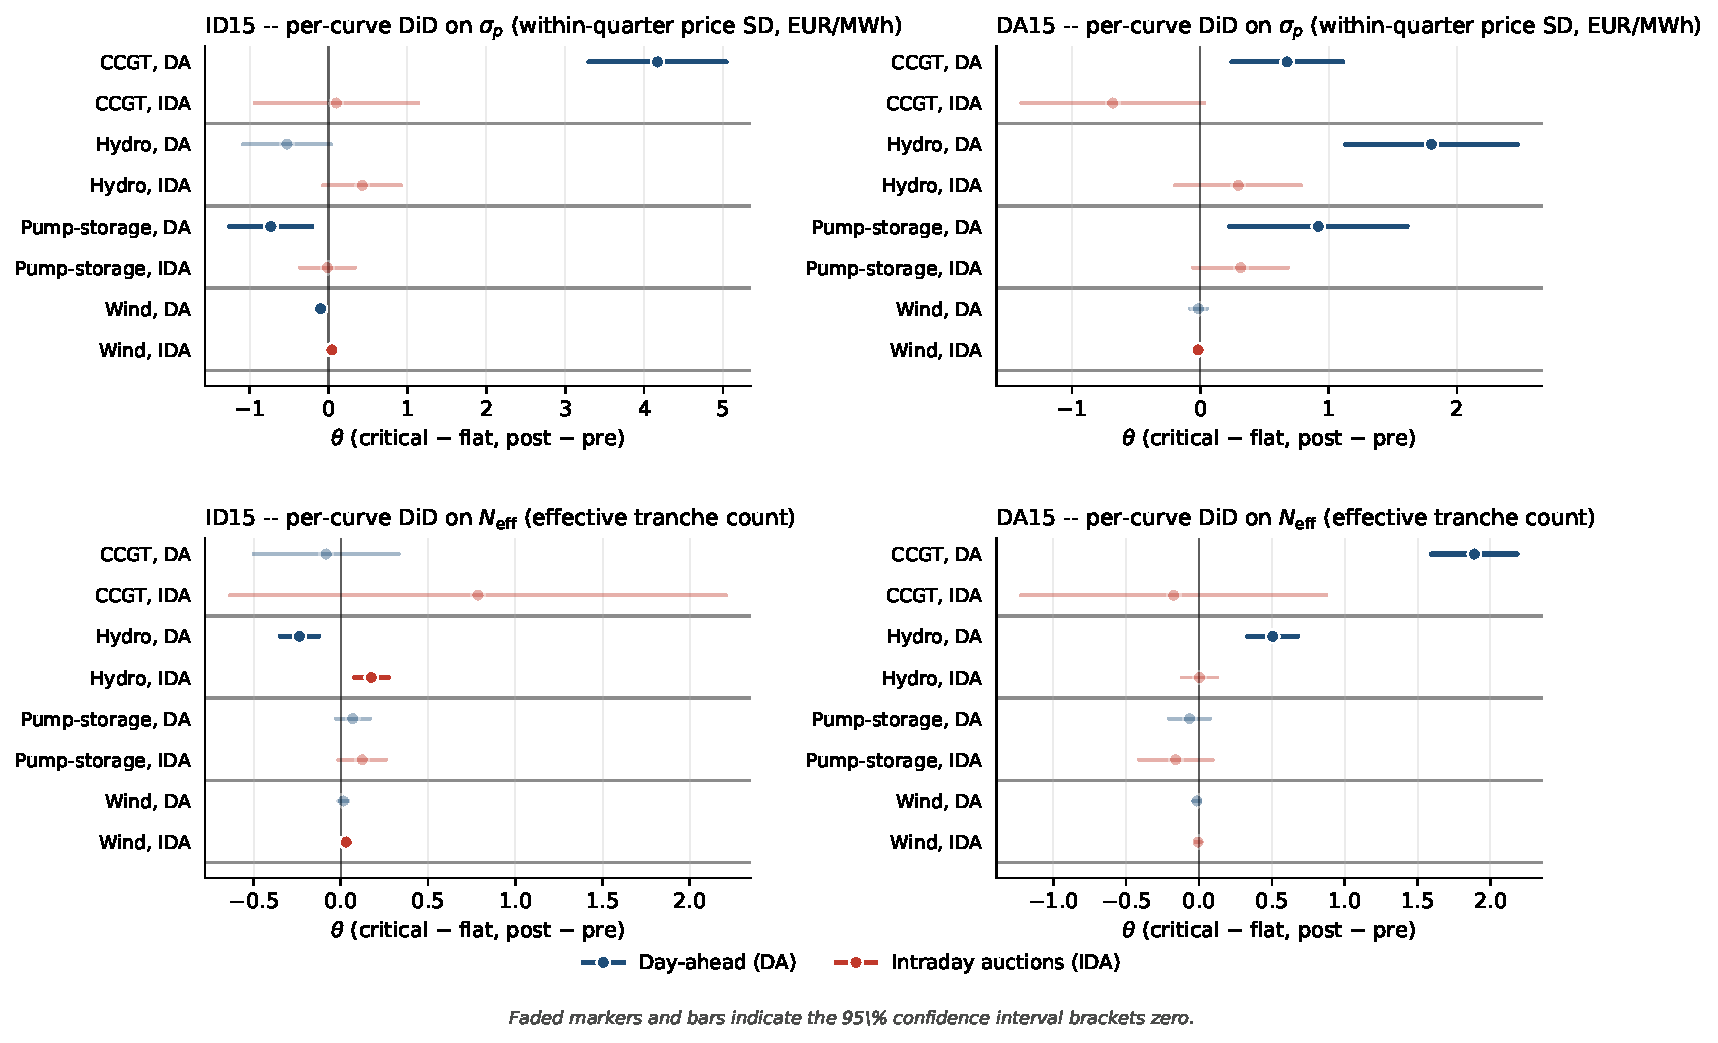
\includegraphics[width=\linewidth]{fig_sigma_p_forest.pdf}
\caption{\textbf{Spec~C per-curve DiD on bid-shape outcomes at the window-specific p90 bandwidth.} \emph{Top row:} $\sigma_p$ DiD (within-quarter price SD); \emph{Bottom row:} $N_{\text{eff}}$ DiD (effective tranche count). \emph{Left column:} ID15. \emph{Right column:} DA15. Each row inside a panel is one (tech, market) cell; blue = day-ahead, red = intraday auctions. Faded markers indicate the 95\% CI brackets zero. Bandwidth $h$ varies by (window, market): ID15 uses h=50 (DA) / h=62 (IDA); DA15 uses h=50 (DA) / h=58 (IDA). The picture is genuinely market-specific: ID15's effects concentrate in IDA $N_{\text{eff}}$ (more granular intraday ladders) and DA CCGT $\sigma_p$ (anticipation-channel widening); DA15's effects concentrate in DA across all dispatchables, with CCGT IDA $\sigma_p$ tightening (substitution into DA).}
\label{fig:sigma-p-forest}
\end{figure}

\section*{5. Takeaway: granularity is a strategic-latitude reveal}
\addcontentsline{toc}{section}{5. Takeaway: granularity is a strategic-latitude reveal}
\phantomsection\label{sec:summary}

A market-microstructure reform that simply increases trading-period resolution acts not as a uniform technology shock but as a \emph{strategic-latitude reveal}. It does not change marginal costs, capacity, or who is in the market. It changes who has room to discriminate within the hour and where --- and the equilibrium response traces exactly that, with strategic firms (CCGT, hydro, pump-storage) restructuring bids in critical hours, operational firms (wind and solar aggregators) using the finer grid uniformly to manage imbalance, and both rippling across the sequential markets through cross-market anticipation.

\textbf{\emph{Does granularity amplify market power?} The wholesale-price evidence runs the other way}: intraday clearing prices fall sharply under ID15 and day-ahead prices co-move down via cross-market anticipation, while the day-ahead/intraday wedge keeps its mean at zero. The strategic engagement we document is not rent extraction at consumer expense --- it is firms competing more granularly. More tranches in critical hours expose more of the competing tier to within-hour competition rather than averaging it into a single hourly clearing.

\textbf{\emph{Does it harm consumers?} Direct: wholesale prices fall, so the auction channel is consumer-favourable}. System-wide: the granularity reforms compress the up-direction adjustment-cost channels REE has to call --- real-time redispatch and aFRR\footnote{aFRR (automatic Frequency Restoration Reserve) is a continuous balancing service: units that have committed an aFRR band are automatically signalled to ramp up or down within seconds to correct system frequency deviations.} reserve activations both shrink across the reform sequence (\hyperref[fig:efficiency_gains]{Appendix~C.3, Figure~\ref*{fig:efficiency_gains}}). The only channel that grows across the same window is Fase~I\footnote{Fase~I is REE's primary up-redispatch market: after the OMIE day-ahead auction clears, REE may need extra generation in specific zones (to ease grid congestion or restore voltage margins) and procures it through a separate pay-as-bid restriction offer.} up-redispatch, but this is the response to the post-blackout reinforced-operation regime, not to MTU15: the two policies overlap calendar-wise but operate on different mechanisms (\hyperref[fig:ree_intervention_by_tech]{Appendix~C.4, Figure~\ref*{fig:ree_intervention_by_tech}}). Net of the reforzada-driven Fase~I growth, the granularity reforms are cost-reducing for the system.

A deeper question is whether the March 2025 ID15 reform was in some way responsible for the April 2025 blackout, and therefore indirectly for the post-blackout rise in consumer prices through reforzada-driven REE restrictions. The most authoritative investigation on the incident --- the ENTSO-E Expert Panel's final report --- does not list ID15 as a contributing factor: its root-cause tree points to voltage- and reactive-power-control failures (renewable plants operating at fixed power factor, manually-operated shunt reactors, divergent overvoltage protection settings, converter-driven instability, absence of power-system stabilisers on several large units) \citep{entsoe_blackout_iberia_2026}.

Anecdotally, the parallel CNMC report does flag the move to quarter-hourly trading as one contributor to the abrupt voltage variations observed in the months around the incident \citep[p.~44]{cnmc_blackout_recommendations_2026}:
\begin{quote}
\itshape It is worth recalling that the implementation of the 15-minute trading unit in the Spanish intraday market was completed on 18 March 2025, one month before the incident, with the entry into force of quarter-hourly trading in both the intraday auctions and the continuous intraday market. The implementation was carried out within the framework of the European intraday coupling projects in line with Regulation (EU) 2017/2195. The evolution to quarter-hourly trading and settlement has made the appearance of transitions between negative and positive prices increasingly frequent, leading to strong changes in production volumes in certain zones.\footnote{Original (CNMC report, p.~44): \emph{``A este respecto, cabe recordar que el proceso de implantaci\'on de la unidad de negociaci\'on de 15 minutos en el mercado intradiario espa\~nol se complet\'o el 18 de marzo de 2025, 1 mes antes del incidente, con la entrada en vigor de la negociaci\'on cuarto-horaria tanto en las subastas intradiarias como en el mercado intradiario continuo. La implementaci\'on se realiz\'o en el marco de los proyectos europeos de acoplamiento intradiario en coherencia con el Reglamento (UE) 2017/2195. La evoluci\'on a una negociaci\'on y liquidaci\'on de productos cuarto horarios ha hecho cada vez m\'as frecuente la aparici\'on de transiciones entre precios negativos y positivos que conducen a fuertes cambios del volumen de producci\'on en determinadas zonas.''}}
\end{quote}

\textbf{Answering this question is beyond the scope of this thesis} --- it requires electrical-engineering knowledge we do not have --- but it points to a strong research gap: the ENTSO-E report may be identifying the proximate technical triggers but not engaging with whether the market-microstructure reforms contributed to the macro-conditions (frequent within-hour swings, converter-driven volatility under fixed-power-factor RES dispatch) that made the system fragile enough for those triggers to cascade. The CNMC's anecdotal flag points exactly there.

\newpage

\bibliographystyle{plainnat}
\addcontentsline{toc}{section}{References}
\bibliography{../paper/references}

\newpage

\appendix

\section*{Appendix A. Robustness}
\addcontentsline{toc}{section}{Appendix A. Robustness}
\phantomsection\label{sec:robustness}

A few caveats up front: bid-shape DiDs in a market this complex (overlapping reforms, regulatory regime changes, weather-driven dispatch) will not deliver textbook causal cleanliness on every cell. The robustness checks below are designed to flag where the headline reading is solid and where it rests on shakier ground, not to deliver a single ``did identify'' verdict.

\subsubsection*{A.1. Pre-trend placebo --- the headline check \textnormal{(partially supportive)}}\phantomsection\label{sec:5b}
\addcontentsline{toc}{subsection}{A.1. Pre-trend placebo --- the headline check (partially supportive)}
A pre-only midpoint placebo splits each reform's pre-window at its midpoint and runs a fake critical-flat DiD on the same outcome. ID15 IDA dispatchable $\sigma_p$ placebos all bracket zero --- the ID15 bid-shape findings rest on a clean pre-trend. For DA15 day-ahead: hydro $\sigma_p$ placebo is clean, CCGT $\sigma_p$ placebo runs opposite the headline (so de-trending strengthens it), and pump-storage $\sigma_p$'s placebo exceeds the headline DiD --- not separable from a pre-existing trend.

\subsubsection*{A.2. Hour-class falsification (midday vs.\ flat) \textnormal{(supportive)}}\phantomsection\label{sec:5a}
\addcontentsline{toc}{subsection}{A.2. Hour-class falsification (midday vs.\ flat) (supportive)}
A midday-vs-flat falsification gives sign-stable but smaller-magnitude DiDs at $p_{90}$: the reform reshapes the entire non-flat zone, consistent with \hyperref[sec:4-specB]{\S~4.B}. The cleaner critical-vs-flat contrast remains the headline because flat hours are the unambiguous within-day control.

\subsubsection*{A.3. Cross-border and reforzada --- the two natural confounds \textnormal{(supportive)}}\phantomsection\label{sec:5c}\phantomsection\label{sec:5d}
\addcontentsline{toc}{subsection}{A.3. Cross-border and reforzada --- the two natural confounds (supportive)}
SIDC/XBID also moved to 15-min on the same date as ID15 --- a sibling treatment on the same reform, not an OVB: adding hourly cross-border net flow as a control on ID15 IDA $\sigma_p$ leaves the per-tech DiDs essentially unchanged. The reforzada regulatory stance acts on the \emph{level} of Fase~I up-redispatch, not its \emph{within-hour SD}: reforzada parks capacity in the scarcity tier and recalls it through restriction offers (\hyperref[sec:context]{Appendix~C}), while MTU15 reshapes the competing tier within the band --- two non-overlapping mechanisms.

\subsubsection*{A.4. Per-CCGT-firm decomposition of the DA15 $\sigma_p$ widening \textnormal{(heterogeneity description, not a validation)}}
\addcontentsline{toc}{subsection}{A.4. Per-CCGT-firm decomposition of the DA15 $\sigma_p$ widening (heterogeneity description, not a validation)}
The pooled DA15 CCGT day-ahead $\sigma_p$ widening of \hyperref[sec:4i]{\S~4.C.1} is driven primarily by Naturgy and to a lesser extent Iberdrola; Endesa and EDP-HC do not contribute. The Naturgy effect is not a flat-baseline artefact: $\sigma_p$ rises in both arms but more in critical hours. The bid-shape engagement is therefore not Big-4-uniform; it concentrates in the two firms that have historically been most active in the day-ahead competing tier.

\subsubsection*{A.5. Bandwidth $h$ \textnormal{(supportive at $p_{90}$, problematic at wider bandwidths)}}\phantomsection\label{sec:5e}
\addcontentsline{toc}{subsection}{A.5. Bandwidth $h$ (supportive at $p_{90}$, problematic at wider bandwidths)}
$p_{90}$ isolates the competing tier and excludes the parked tier above the ceiling (a non-strategic placeholder, \hyperref[sec:context]{Appendix~C}). Including the parked tier would bias $\sigma_p$ upward by a measurement-driven cross-tier spread. The picture is robust to small shifts around $p_{90}$; at much wider bandwidths, CCGT $\sigma_p$ magnitudes inflate and several DiD coefficients flip sign because the cross-tier spread moves across the cutover for reasons unrelated to within-tier bidding. The IDA bandwidth pools the three sessions; session~3 has a materially wider $p_{90}-p_{50}$ than sessions~1--2, but a session-specific $h$ cannot flip signs --- the per-session BSTS in \hyperref[sec:5f]{Appendix~A.6} shows the price-level effect is uniform across sessions.

\subsubsection*{A.6. Per-IDA-session BSTS \textnormal{(supportive)}}\phantomsection\label{sec:5f}
\addcontentsline{toc}{subsection}{A.6. Per-IDA-session BSTS (supportive)}
Running Spec~A separately on each IDA session's daily mean price (Table~\ref{tab:bsts-per-session}) confirms session symmetry: the ID15 placebo-net drop is essentially identical across S1, S2, S3, and the DA15 IDA-side rise sits in a narrow positive band. ID15 placebo uses the 2026 same-calendar window (the 2024 placebo predates the 6$\to$3 IDA reform and is not session-comparable).

\begin{center}
\footnotesize
\setlength{\tabcolsep}{6pt}
\begin{tabular}{l l c c c}
\toprule
\textbf{Reform} & \textbf{Session} & \textbf{Effect (real)} & \textbf{Placebo} & \textbf{Placebo-net} \\
\midrule
\multirow{3}{*}{ID15 IDA} & S1 & $-79.8^{***}$ & $-16.1^{*}$ & $-63.7^{***}$ \\
                          & S2 & $-79.9^{***}$ & $-11.4$      & $-68.5^{***}$ \\
                          & S3 & $-81.9^{***}$ & $-8.4$       & $-73.5^{***}$ \\
\addlinespace
\multirow{3}{*}{DA15 IDA} & S1 & $15.4^{***}$  & $3.9$        & $11.5^{**}$   \\
                          & S2 & $14.4^{***}$  & $-1.8$       & $16.2^{***}$  \\
                          & S3 & $19.0^{***}$  & $10.6^{**}$  & $8.4$         \\
\bottomrule
\end{tabular}
\captionof{table}{\textbf{Per-IDA-session BSTS on daily clearing prices.} BSTS posterior means in EUR/MWh; tail-probability stars $^{*}p{<}0.10$, $^{**}p{<}0.05$, $^{***}p{<}0.01$. ID15 placebo is the 2026 same-calendar window (3 sessions, matching real). DA15 placebo is 2024 same-calendar (3 sessions). Same windows and covariates as Spec~A. Session symmetry implies pooling across sessions in the headline IDA BSTS is innocuous: a session-specific bandwidth would not change the level conclusion.}
\label{tab:bsts-per-session}
\end{center}

\section*{Appendix B. \textcolor{red}{Continuous-market response at the three structural reforms}}
\addcontentsline{toc}{section}{Appendix B. Continuous-market response at the three structural reforms}
\phantomsection\label{sec:continuous}

\paragraph{Specification.} BSTS counterfactual on daily ES-leg continuous-market series with wind+solar+gas covariates and a weekly seasonal cycle (same setup as \hyperref[sec:bsts]{\S~3.A}). Quantity outcomes are reported in \emph{energy} (MWh per trade $\times$ delivery hours, summed per day) rather than raw MW sums --- post-MTU15 each clock-hour holds four 15-min contracts where pre-MTU15 it held one 60-min contract, so a raw MW sum would be mechanically inflated. The volume-weighted price is energy-weighted. Three reform cutovers (ISP15 2024-12-11, ID15 2025-03-19, DA15 2025-10-01), each with a 2023/2024 same-calendar placebo.

\begin{center}
\footnotesize
\setlength{\tabcolsep}{4pt}
\begin{tabular}{l l r r r}
\toprule
\textbf{Reform} & \textbf{Outcome} & \textbf{Real} & \textbf{Placebo} & \textbf{Placebo-net} \\
\midrule
\multirow{3}{*}{ISP15}  & $n_{\text{trades}}$/day  & $-3{,}120^{***}$ & $-1{,}231^{***}$ & $-1{,}889$ \\
                        & GWh/day                  & $-3.85^{*}$      & $-2.23^{**}$     & $-1.62$ \\
                        & VW-price (EUR/MWh)       & $-15.1$          & $-27.4^{***}$    & $12.3$ \\
\addlinespace
\multirow{3}{*}{ID15}   & $n_{\text{trades}}$/day  & $22{,}335^{***}$ & $1{,}381^{*}$    & $20{,}954^{***}$ \\
                        & GWh/day                  & $-7.19^{***}$    & $6.72^{***}$     & $-13.91^{***}$ \\
                        & VW-price (EUR/MWh)       & $-80.1^{***}$    & $-14.1^{***}$    & $-66.0^{***}$ \\
\addlinespace
\multirow{3}{*}{DA15}   & $n_{\text{trades}}$/day  & $5{,}018^{**}$   & $257$            & $4{,}761$ \\
                        & GWh/day                  & $3.85^{***}$     & $-1.35$          & $5.20^{**}$ \\
                        & VW-price (EUR/MWh)       & $4.7$            & $-4.7$           & $9.4$ \\
\bottomrule
\end{tabular}
\captionof{table}{\textbf{Continuous-market response at the three structural reforms.} BSTS posterior means; tail-probability stars $^{*}p{<}0.10$, $^{**}p{<}0.05$, $^{***}p{<}0.01$. Placebo-net joint significance based on independent posteriors propagating two variances.}
\end{center}

\subsubsection*{B.1. ISP15 (settlement-only): a methodological null}\addcontentsline{toc}{subsection}{B.1. ISP15 (settlement-only): a methodological null}
ISP15 changed how REE settles imbalance positions (60$\to$15 min) but left the OMIE continuous-market contract grid unchanged --- traders still bought and sold hourly delivery contracts. A null effect is the right prediction here. Raw trade count and energy turnover both fall, but the same drift appears in the 2023 placebo (settlement bookkeeping innovations are not the source), and all three placebo-net intervals bracket zero. A settlement-only reform shows nothing on contract-structure outcomes --- the specification reads the reform where it lives.

\subsubsection*{B.2. ID15 (60$\to$15 min): the structural continuous-market reform}\addcontentsline{toc}{subsection}{B.2. ID15 (60$\to$15 min): the structural continuous-market reform}
Pre-reform, each clock-hour of delivery hosted a single 60-min contract; post-reform, four 15-min contracts. The three outcomes move accordingly:
\begin{itemize}\setlength{\itemsep}{1pt}
\item \emph{Trade count.} Each hour now offers four matching opportunities instead of one, so the trade-count surge is mechanical at first order --- but informative: it confirms participants actually \emph{used} the new finer grid rather than continuing to aggregate to the hourly contract.
\item \emph{Energy turnover.} Placebo-net is \emph{negative}: more contracts, each smaller, and total energy changing hands drops. Two reasons: some hourly counterparties drop out when they don't see a 60-min match on offer, and some dispatchable bidding migrated into the now-finer IDA auctions instead (\hyperref[sec:4v]{\S~4.B.1}).
\item \emph{Volume-weighted price.} The continuous market clears in equilibrium with the auctions, so the ID15 cutover price drop on auction-cleared prices (\hyperref[sec:4ii]{\S~4.A.1}) shows up here too --- the cross-market spillover documented for ID15.
\end{itemize}

\subsubsection*{B.3. DA15: a smaller, indirect continuous-market effect}\addcontentsline{toc}{subsection}{B.3. DA15: a smaller, indirect continuous-market effect}
DA15 does not touch the continuous-market contract grid (already 15-min post-ID15); only the day-ahead \emph{reference price} that continuous traders watch becomes finer. With a finer DA reference, traders reposition more aggressively in continuous: daily GWh up (joint 95\% retains), trade count borderline, price effect statistical noise. DA15's continuous-market footprint is incremental and proportional to how much tighter the day-ahead reference now is --- not a structural break, as expected from a reform that touches the reference market but not the continuous-market contract architecture.

\section*{Appendix C. Two market-structure facts that frame the bidding evidence}
\addcontentsline{toc}{section}{Appendix C. Two market-structure facts that frame the bidding evidence}
\phantomsection\label{sec:context}

\subsubsection*{C.1. The two-tier CCGT bid curve and the day-ahead/intraday contrast}\addcontentsline{toc}{subsection}{C.1. The two-tier CCGT bid curve and the day-ahead/intraday contrast}
Every Big-4 CCGT fleet runs a two-tier day-ahead offer: a low \emph{competing} tier near marginal cost and a high \emph{parked} tier above the clearing-price ceiling. Withholding is firm-wide, not a Naturgy story. The same fleets bid a single competitive tier with negligible withholding in the intraday auction, after Fase~I has cleared. A unit's marginal cost does not change between two auctions hours apart. The parked tier is a placeholder rather than a Fase~I bid: Fase~I up-redispatch is settled through a separate restriction offer submitted to REE.\footnote{Procedure PO 3.2, settlement PO 14.4 ap.~20.1; see also \citet{boe_a_2025_5342,boe_a_2025_13076}. Earlier drafts of this memo conflated the two; the distinction justifies measuring bid shape and bid levels in the competing tier only, which is what the window-specific $p_{90}$ bandwidth in \hyperref[sec:setup]{\S~1} achieves.} MTU15-DA grants CCGT a within-hour degree of freedom over its competing tier; the CCGT auction-cleared scale-up in \hyperref[sec:4iii]{\S~4.A.2} is the competing tier expanding into the four quarters of each peak hour.

\subsubsection*{C.2. Market concentration migrated from wholesale to ancillary services}\addcontentsline{toc}{subsection}{C.2. Market concentration migrated from wholesale to ancillary services}
Wholesale-market HHI hovers around 1\,100 over 2016--2024 (below the moderate-concentration threshold of 1\,500) and falls mid-day when solar peaks (solar is less concentrated than the Big-3). Day-ahead restrictions upward HHI above 4\,000; deviations upward above 6\,000; tertiary upward around 5\,000. Median of 4 firms with accepted upward restrictions bids. As renewables eroded wholesale-market power, technical and locational requirements concentrated the ancillary markets that absorb their variability.

\subsubsection*{C.3. Granularity shrinks some channels; reforzada inflates others}\addcontentsline{toc}{subsection}{C.3. Granularity shrinks some channels; reforzada inflates others}
After the OMIE auction clears, REE may still need to act on the schedule in several ways --- buying MW from units to dispatch them \emph{up} (when the system runs short or needs voltage support), or paying units to reduce output \emph{down} (including renewable curtailment when there is excess supply). The four UP channels and four DN channels are all costs that REE pays to providers. Figure~\ref{fig:efficiency_gains} stacks them by regime, using the six reform-window regimes of Figure~\ref{fig:bid_internal:timeline} --- UP at the bottom (solid), DN on top (hatched) --- and shades pre-blackout regimes blue and post-blackout regimes (reforzada in force) red, because the granularity reforms and the reforzada response operate on different mechanisms and should not be conflated.

The cleanest evidence for the granularity channel is \emph{within the pre-blackout zone}: from ISP15-win to DA60/ID15-pre (the 40-day MTU15-IDA window before the April 2025 blackout), total per-day ajuste cost drops from $\sim$EUR\,16M to $\sim$EUR\,14M, driven by real-time redispatch falling by roughly a third, aFRR up shrinking by about half, and the down-direction channels shrinking in parallel. With a quarter-level cleared schedule, the auction itself absorbs within-hour variation that previously had to be cleaned up ex post, in either direction.

The channel is most visible in renewables. Solar aggregators exploit granularity in midday hours --- when solar actually produces --- by committing to four quarter-level schedules that track cloud-cover variation instead of a single hourly commitment. The Spec~A finding that solar cleared MW shifts into midday DA under DA15 (\hyperref[sec:4-renewable]{\S~4.A.3}) is the auction-side footprint of exactly this channel: less within-hour mismatch upstream, less imbalance for REE to absorb downstream.

\begin{figure}[h]
\centering

\includegraphics[width=\textwidth]{../../figures/working/efficiency_gains_timeseries.pdf}
\caption{\textbf{Evolution of daily ajuste-cost composition (EUR M / day, $14$-day rolling mean): UP (solid) and DN (hatched) stacked.} All eight channels are gross costs REE pays providers, so all are stacked positive. UP layers at the bottom (REE buys MW to dispatch up), DN layers on top (REE pays units to come down, including renewable curtailment under Fase~I dn and Fase~II dn). Background shading splits the timeline into pre-blackout (blue) and post-blackout / reforzada (red); vertical dotted lines mark the five reform dates of Figure~\ref{fig:bid_internal:timeline}. The granularity-only signal is clearest in the pre-blackout zone: TR up (blue) starts large and falls sharply after MTU15-IDA; aFRR follows. Post-blackout, Fase~I up (red) balloons (CCGT dispatched up for voltage support) and the DN side grows (renewables curtailed to make room); the granularity channels continue to shrink, but the reforzada-driven growth dominates the headline total. TR dn is reported in the source data net of a small refund; we take its absolute value here for the gross-cost reading. \emph{Figures are raw per-day rates with a $14$-day rolling mean for readability --- not seasonally adjusted.}}
\label{fig:efficiency_gains}
\end{figure}

In the post-blackout regimes, the headline total \emph{rises} despite the granularity channels continuing to shrink. Fase~I up balloons by $\sim$EUR\,5M/day (CCGT dispatched up for voltage support) and Fase~II dn grows by $\sim$EUR\,2--3M/day (units, including renewables, curtailed to make room). These are reforzada-driven, not MTU15. The granularity channels within the post-blackout zone keep shrinking (TR up falls further from DA60/ID15 post to DA15/ID15 once the day-ahead grid moves to 15-min), but they are overwhelmed in the headline total by the reforzada growth. A cost analysis that does not separate the two policies will read the MTU15 reforms as a net cost increase, when the granularity channels themselves are cost reducers in both directions and the post-blackout reinforced-operation regime is the actual driver of the headline cost rise.

\subsubsection*{C.4. The reforzada cost increase concentrates on CCGT}\addcontentsline{toc}{subsection}{C.4. The reforzada cost increase concentrates on CCGT}
The post-blackout REE intervention is technology-specific. Decomposing weekly dispatch into its components --- the day-ahead-cleared base (PDBC), bilateral executions, and the post-DA top-up routed through IDA and REE real-time redispatch --- the CCGT panel of Figure~\ref{fig:ree_intervention_by_tech} shows the day-ahead-cleared layer (blue) collapsing post-blackout while the IDA+REE-RT layer (red) balloons. Other technologies are largely flat across the same window.

\begin{figure}[h]
\centering
\includegraphics[width=\textwidth]{../../figures/working/fig_q_components_by_tech_weekly.pdf}
\caption{\textbf{Weekly three-component decomposition of dispatch, by technology.} PDBC (blue, day-ahead-cleared) $+$ bilateral executions (green) $+$ IDA $+$ REE real-time top-up (red) $=$ final post-IDA dispatch (black). CCGT's day-ahead-cleared layer collapses post-blackout while the IDA $+$ REE-RT layer balloons; other technologies are flat. Vertical guides mark MTU15-IDA, the April 2025 blackout, and MTU15-DA.}
\label{fig:ree_intervention_by_tech}
\end{figure}

This per-technology pattern is the cleanest evidence that the reforzada cost increase is a separate policy effect from the granularity reforms: a granularity reform that touched all bid-side firms equally would not produce a CCGT-only intervention pattern. The day-ahead CCGT cleared scale-up of \hyperref[sec:4iii]{\S~4.A.2} (DA15 only, critical hours) sits alongside this REE-intervention story: both are CCGT-side responses to the operational environment, but the granularity-driven response is competitive-clearing (and consumer-favourable) while the reforzada-driven response is REE-paid redispatch.

\end{document}
